\documentclass[11pt,a4paper]{article}
\usepackage[T1]{fontenc}
\usepackage[utf8]{inputenc}
\usepackage{lmodern,amsmath,amssymb,amsthm,mathtools,bm}
\usepackage[margin=24mm,headheight=15pt]{geometry}
\usepackage{graphicx,booktabs,array,microtype,xcolor,fancyhdr}
\usepackage[numbers,sort&compress]{natbib}
\usepackage{hyperref}
\hypersetup{colorlinks=true,linkcolor=blue!45!black,citecolor=blue!45!black,urlcolor=blue!45!black,
pdftitle={Blackhole Tracker: BHSM Boundary Interpretation of Compact-Lens Mass, Motion, and Conditional Response},pdfauthor={Norman P. Carberry},
pdfsubject={Formal source and reviewer repository: https://github.com/ncarberry64/Berger-Hopf-Standard-Model},pdfkeywords={BHSM, Blackhole Tracker, gravitational lensing, boundary response}}
\pagestyle{fancy}\fancyhf{}
\fancyhead[L]{\small Blackhole Tracker: BHSM boundary interpretation}
\fancyhead[R]{\small Research article}\fancyfoot[C]{\thepage}
\setlength{\parskip}{.3em}\setlength{\parindent}{1em}
\setlength{\emergencystretch}{3em}
\renewcommand{\topfraction}{.93}\renewcommand{\textfraction}{.06}
\newtheorem{theorem}{Theorem}\newtheorem{proposition}{Proposition}
\newtheorem{corollary}{Corollary}\newtheorem{lemma}{Lemma}
\newcommand{\tr}{\operatorname{tr}}
\newcommand{\asinh}{\operatorname{asinh}}
\title{\textbf{Blackhole Tracker: BHSM Boundary Interpretation of Compact-Lens Mass, Motion, and Conditional Response}}
\author{Norman P. Carberry\\\small Independent Researcher, Oconomowoc, Wisconsin, USA\\
\small \href{mailto:carberry8878130@hotmail.com}{carberry8878130@hotmail.com}\\
\small ORCID: \href{https://orcid.org/0009-0000-6650-3485}{0009-0000-6650-3485}}
\date{}
\begin{document}
\maketitle
\begin{center}\small Research article for \emph{Galaxies}: Strong Gravitational Lens Modeling\end{center}
\begin{abstract}
Blackhole Tracker interprets compact-lens inference as Berger--Hopf Standard
Model (BHSM) gravitational surface topography, counting one
exterior once. App, command-line, Python and notebook interfaces support
resolved pairs and native photometry. A frozen pilot processes
100 OGLE-III events and 76\,344 measurements: 89 fail its adequacy screen,
eleven are not rejected and two pass stricter archival follow-up criteria.
An atlas adds 59 published parallax events, retaining 155 distinct
source/event directions and failed assessments. Three qualified or disputed
targets remain unconfirmed.
Mass, lens position, distance and absolute motion remain unresolved;
duration is not mass. A joint benchmark retains 12\,521 photometric
measurements and 21 two-coordinate HST positions: three Gaussian noise
candidates fail residual checks; a normalized Student experiment remains
numerically unresolved. Corrections remove numerical-reference dependence,
admit physical nuisance profiles and preserve unavailable motion uncertainties.
A frozen synthetic study retains 4\,608 datasets and 4\,736 fits; three
photometric uncertainty-calibration tests fail alongside successful conditional
resolved controls. The optional scalar--tensor calculation bounds retained
boundary states, but two projected modes vanish and the leading response
is degenerate with shear. The product supports auditable screening and
conditional response tests. No new black-hole identification, independent
known-black-hole recovery, measured BHSM core dynamics, independently
detected R1 deformation or horizon classification is established.
\end{abstract}
\noindent\textbf{Keywords:} strong gravitational lensing; compact objects;
microlensing; native photometry; scalar--tensor gravity; boundary response; identifiability

\section{Introduction: the Blackhole Tracker question}

BHSM motivates a hunt for gravitational topography of the hypersurface
and for observations that distinguish different envelopments. The author
describes this as a hunt on the hypersphere surface
\cite{CarberryEnvelopmentSearch2026}. Here the search becomes operational
through one projected optical response, its measurable differentials and
explicit tests of which configuration distinctions survive the available
data. Compact lenses and extended, dark-matter-like interpretations require
their own response models and evidence; a shared exterior remains counted
once. Section~\ref{sec:envelopment-comparison} makes that comparison precise
without assigning an unmeasured microscopic boundary or a global radius.

Lensing already measures the mass and motion of dark compact objects.
Astrometric microlensing has been used to infer an isolated stellar-mass
black-hole candidate's properties \cite{Sahu2022}; joint astrometry and
parallax separate familiar mass, distance and proper-motion combinations.
Moving dark structures also motivate multi-source astrometric templates
\cite{VanTilburg2018}, and repeated lensed bursts carry motion-dependent
delays \cite{Dai2017}. The product makes this measurement workflow reproducible under an explicit
data contract. Its action-specific question is narrower: can a specified
envelope deformation supply a calculable linked pattern in images, fluxes
and delays, and which parts survive an ordinary lens fit?

BHSM organizes its research around boundary geometry, constrained actions
and envelope matching. That language does not by itself fix a metric,
surface state or optical coefficient. An ordinary gravitational potential
may already describe the same boundary contribution. We therefore use a
declared Einstein/GHY sector for the ordinary fit and a single
scalar--tensor action for the optional R1 response, counting each
physical contribution once. The name
\emph{Blackhole Tracker} denotes the proposed application to a candidate
compact dark source. All rays in this paper lie far outside a declared
worldtube, itself far outside the gravitational radius. Lensing on that
domain does not establish a horizon or identify the compact interior.

The real-observation extension adds a separate unresolved-photometry
route and freezes its selection, likelihood and all-event reporting
before fitting. It preserves the downloaded measurements instead of
forcing them into a resolved-image contract. Its observational outcome is
event screening with mass unresolved, including a retained negative
benchmark result; it does not manufacture a black-hole classification.

The central deliverable is a usable research product with an ordinary
compact-lens tracking mode and an optional conditional boundary-response
mode. The ordinary fit is interpreted in the recovered BHSM Einstein/GHY
sector through the same exterior mass and its boundary representation;
this interpretation does not add another gravitational contribution.
The new theoretical result is a uniform sufficient admission bound
on the normalized quadrupole throughout the retained R1 exterior. The
optical calculation identifies exact blind directions and demonstrates
why a working compact-mass track need not detect an envelope. A separate
nonlinear product validation tests mass/motion recovery, full covariance,
limited interval calibration and unsuccessful controls. These statements
are independent of accepting a departure from GR; their action-specific
application remains conditional.

\subsection{Recovered record and scope of the new calculation}

A finite recovery covered relevant local Git branches/worktrees, research
files in Downloads and Documents, selected members of a mounted BHSM
backup, and accessible excerpts of the conversation \emph{Strong Lensing
Paper Plan}. The source map and content hashes are distributed with the
calculation. This is actual access to selected material, not comprehensive
recall of every conversation or archive.

The earlier angular paper was recovered from
\texttt{BHSM\_Angular\_Lensing\_Reproducibility.zip}, SHA256 beginning
\texttt{84786b6b905ae1e2}. Its round closed-background, nine-harmonic,
six-coordinate calculation is preserved separately. Its illustrative
fixed-physical-source SIS delay shift, $-0.353216090$ s against a
$7.753621449$ d baseline, is a conditional chosen state, not a selected
black-hole signal. The earlier observational HE0435 paper and its failed
or incomplete observational tests are also preserved. No such data are
used here. A separate Hopf-charge result is retained as supporting
research rather than made the central tracker claim.

\begin{table}[t]
\centering\small
\caption{Recovered objects relevant to the tracker. ``Not located'' refers
only to the searched record. Exact paths/hashes are in the source map.}
\begin{tabular}{p{.28\linewidth}p{.63\linewidth}}
\toprule Object & Scientific status and use\\\midrule
R1 covariant action and homogeneous background & Conditional effective
realization; archived source and hashes recovered and replayed. Supplies
the local coefficients used here.\\
Compact-source cubic reduction & Recovered action-derived quasi-static
constraints and regular-body branch. Re-derived and checked here with
general exterior scalar flux.\\
BHSM black-hole/surface drafts & Surface identities and proposed flux
parameters recovered. Horizon selection of the R1 exterior flux and
causal deformation response not established by those objects.\\
Microscopic constrained Hessian/Schur work & Actual local response machinery
recovered; an evaluated normalized microscopic-to-cosmological optical
map was not located.\\
Fixed external environment & Seven action-owned interface variations
remain even when external labels are fixed. This microscopic prescription
does not fix a cosmological or black-hole deformation state.\\\bottomrule
\end{tabular}
\end{table}

The strongest feasible action-specific deformation route is thus a normalized \emph{conditional
effective-action} calculation. We do not substitute a familiar surface
mass identity for the missing horizon problem. The spherical flux is
kept as an exterior matching datum; the physical state remains free.
The mathematical chain, and the place where it stops, are made explicit.

\section{BHSM interpretation of the reconstructed exterior}
\label{sec:bhsm-interpretation}

The ordinary lens fit is part of the BHSM interpretation used here.
It reconstructs the effective gravitational exterior of the compact
configuration: its monopole, location, translation and admitted projected
structure. An observable departure from GR is not required for that
interpretation. The recovered BHSM source records explicitly admit an
Einstein/GHY compact-source sector, in which boundary and conventional
gravitational descriptions represent the same exterior contribution.
We use that declared sector without promoting it into a unique
microscopic derivation of every fitted parameter.

Let $\mathcal C$ denote a configuration described in the BHSM framework,
and let $W_{\mathcal C}=\Phi_{\mathcal C}+\Psi_{\mathcal C}$ be its
Weyl potential in the stated weak-metric convention. The forward map is
\begin{equation}
 \mathcal C\longmapsto W_{\mathcal C}
 \longmapsto\psi_{\mathcal C}
 \longmapsto(\boldsymbol\theta_+,\boldsymbol\theta_-,
                  \ln R,\Delta t),
 \label{eq:bhsm-optical-interpretation}
\end{equation}
with the supplied distances, clock, angular frame and source positions.
When a source convention writes
$W_{\rm topo}=(\Phi_{\rm topo}+\Psi_{\rm topo})/2$, its contribution to
our full Weyl potential is $2W_{\rm topo}$; this conversion creates no
second physical response.
The fit constrains the projected response represented by
$\psi_{\mathcal C}$. Two descriptions giving the same projected potential
on the relevant image neighborhoods give the same positions,
magnification determinants and relative Fermat delays. Their likelihood
and fitted track are consequently identical. This is a physical
interpretation of the reconstructed exterior, rather than a demand for
an additional force or a second mass contribution.

\begin{table}[tbp]
\centering\small
\caption{Interpretation dictionary for the ordinary optical fit. All
entries remain conditional on the supplied geometry and finite lens model.}
\label{tab:bhsm-interpretation}
\begin{tabular}{@{}p{.23\linewidth}p{.71\linewidth}@{}}
\toprule
Fitted quantity & BHSM interpretation and what is constrained\\\midrule
Optical mass $M_{\rm opt}$ & Effective gravitational monopole of the
represented configuration. It is the point-exterior lens coefficient,
not a measurement of a microscopic constituent mass or a surface energy
without its matching relation.\\
Reference center $\boldsymbol c_0$ & Location of that optical
configuration in the supplied tangent-plane frame.\\
Observer proper motion $\boldsymbol\mu_{\rm obs}$ & Translation of
that same configuration per observer year. It does not measure internal
envelope evolution or select a causal relaxation law.\\
Compact quadrupole & Projected nonspherical structure of the same
exterior; an envelope may be represented by this term when it produces
that potential. The coefficient does not uniquely identify its cause.\\
Shear and convergence & The admitted projected environmental response.
Their interpretation within a BHSM environment does not assign them
uniquely to the tracked compact object.\\\bottomrule
\end{tabular}
\end{table}

The spherical boundary interpretation can be made explicit without
changing the lens equations. In the static Schwarzschild member of the
declared Einstein sector, flat-reference Brown--York energy obeys
\begin{equation}
 E_{\rm BY}(r)=\frac{c^4r}{G}
       \left(1-\sqrt{1-\frac{2GM_{\rm opt}}{c^2r}}\right),\qquad
 M_{\rm opt}=\frac{E_{\rm BY}}{c^2}
       -\frac{G E_{\rm BY}^2}{2c^6r},\quad
 r>\frac{2GM_{\rm opt}}{c^2}.
 \label{eq:bhsm-boundary-mass-interpretation}
\end{equation}
This is the established gravitational boundary construction
\cite{BrownYork1993}, also recovered in the BHSM source record.
The corresponding principal extrinsic-curvature deficit of the enclosing
sphere, relative to its counterpart in a flat spatial slice, and its
inverse mass relation are
\begin{equation}
 \delta k_g(r)=\frac{1-\sqrt{1-2GM_{\rm opt}/(c^2r)}}r,\qquad
 M_{\rm opt}=\frac{c^2}{G}
       \left(r^2\delta k_g-\frac12r^3\delta k_g^2\right).
 \label{eq:bhsm-curvature-mass-interpretation}
\end{equation}
Indeed the two principal curvatures of the enclosing sphere in the static
spatial slice are $\sqrt f/r$, compared with $1/r$ in the flat reference.
This is not its intrinsic Gaussian curvature, which is $1/r^2$ in both
cases at the same areal radius.
For fixed declared $r$, let $f=1-2GM_{\rm opt}/(c^2r)$. Local propagation
of the fitted monopole uncertainty gives
$\sigma_{E_{\rm BY}/c^2}=\sigma_M/\sqrt f$ and
$\sigma_{\delta k_g}=G\sigma_M/(c^2r^2\sqrt f)$.
These are derived representations of the same fitted coefficient, not
independent measurements or a fit of the enclosing radius. If software
uses a computational default for $r$, that choice must remain explicit.
The errors are first-order fixed-radius pushforwards, not finite Gaussian
intervals when a mass range reaches the static-branch boundary $f=0$.
The radius-dependent boundary energy and the conserved monopole are
representations of the same spherical solution. Their contributions
are counted once. The fit does not measure a new worldtube radius, and
changing the enclosing radius in this identity is not physical mass drift.
This static local example does not assert a global cosmological embedding
or continue a static boundary observer through a horizon.

The conditional R1 extension supplies a more specific response relation
from its adopted action, frozen background and supplied matching data.
Its scalar-driven Weyl response may be added only as a distinct term
relative to the already represented reference configuration; an envelope
already absorbed into an ordinary metric multipole cannot be added again
under another name. If two parameterizations produce the same potential,
their degeneracy must be retained. In an R1 fit the reported mass is the
action's metric/source mass parameter; its relation to a point-exterior
$M_{\rm opt}$ must include the scalar contribution to the total potential.
An ordinary quadrupole is not automatically a normalized R1 boundary
amplitude. The forward transfer, state convention and nuisance freedoms
must be specified before that further interpretation is made.

Accordingly a supported mass/motion track is a reconstruction of the
effective BHSM-described optical configuration in the declared sector.
It need not distinguish that interpretation from another theory giving
the same exterior. It does not separately infer the microscopic state,
an astrophysical horizon, scalar flux selection or deformation dynamics.
Those additional inferences require their corresponding source and
matching relations; they are not conditions for retaining the ordinary
fit or for using its mass, location and motion within the stated BHSM
interpretation.

\paragraph{Core and surface: the dated interpretation amendment.}
Norman P. Carberry's 22 October 2026 proposal distinguishes a common
nongeometric core, described by abstract mode weights and algebraic phase
relations, from spacetime-side fields and interfaces
\cite{CarberryCoreSurface2026}. No metric, clock, trajectory, volume or
propagation speed is assigned inside that core. A harmonic label acquires
a physical frequency or length only through a specified realization;
the surface $S^3$ or Berger--Hopf Laplacian is not thereby a core
Laplacian. The existing regular, same-spacetime enclosure carrier and
reciprocal attachment equations retain their own domains. They are not
relabeled as a terminal transfer into the core.

The amendment distinguishes propagating excitations, operative-interface
envelopes and persistent boundary-dominated encapsulations. The inherited
differential is primary in the proposed account; formation, maintenance
and terminal transition are separate questions. Sustained black-hole
conversion, a distinct quiet neutron-star endpoint, quantum loss/regain
of surface manifestation and historical galaxy boundary persistence are
attributed hypotheses, not additional findings of this lens fit. In
particular a proposed terminal channel with zero spacetime daughters
still requires charge/flux accounting and a physical matching law. The
enclosing radius in Eqs.~\eqref{eq:bhsm-boundary-mass-interpretation}--
\eqref{eq:bhsm-curvature-mass-interpretation} is not a measurement of the
proposed hard interface. No new optical term or core parameter follows
from this interpretive update.

\paragraph{What a further core-to-optical calculation must determine.}
There is a useful conditional response criterion, beyond merely naming
a matching relation. Let $\boldsymbol a$ be a declared differentiable
chart of abstract mode data, with its admissible topology specified;
it is distinct from an existing regular child-state coordinate and from
the prescribed R1 boundary amplitudes $a_A$ used elsewhere in this paper.
Let $Q$ collect all regular metric, field and interface data entering
the observable vector $\boldsymbol o$, together with the constraints
and gauge choice. If a physical correspondence specifies
$F_\Sigma(Q,\boldsymbol a)=0$ and
$K=D_QF_\Sigma$ has an appropriate bounded inverse on the declared
constrained physical tangent, differentiation gives
\begin{equation}
 D_{\boldsymbol a}Q=-K^{-1}D_{\boldsymbol a}F_\Sigma,\qquad
 D_{\boldsymbol a}\boldsymbol o
 =-D_Q\boldsymbol o\,K^{-1}D_{\boldsymbol a}F_\Sigma.
 \label{eq:core-optical-conditional-response}
\end{equation}
This form assumes that $Q$ includes every optical input apart from
supplied geometry. If an independently relevant input is omitted, its
explicit $D_{\boldsymbol a}\boldsymbol o|_Q$ term must also be retained.
For the existing linear regular-side constrained response $Ky=f$, the
corresponding operator-derivative identity is
$D_{\boldsymbol a}y=K^{-1}[(D_{\boldsymbol a}f)
 -(D_{\boldsymbol a}K)y]$, with the declared retarded child recovery.
It does not replace an unknown core derivative by a regular child jet.

For the full supplied covariance $C=LL^{\mathsf T}$ and whitened
nuisance Jacobian $N$, the locally retained response is
\begin{equation}
 J_{\rm core}^{\rm prof}
 =(I-NN^+)L^{-1}D_{\boldsymbol a}\boldsymbol o,\qquad
 F_{\rm core}=(J_{\rm core}^{\rm prof})^{\mathsf T}
                  J_{\rm core}^{\rm prof}.
 \label{eq:core-profiled-information}
\end{equation}
The pseudoinverse uses the declared local nuisance rank. Only directions
outside the kernel of this profiled map can be distinguished. Optical
projection nulls cannot be removed by renaming a regular mode a core
harmonic. These equations specify a conditional calculation; the physical
chart/domain and $D_{\boldsymbol a}F_\Sigma$ still have to come from the
core-to-regular correspondence. An unavailable transfer is not a zero
response, and the present software reports no numerical core information
matrix, transition rate or daughter probability.

\paragraph{Prospective discovery use.}
The engine is intended to help identify previously uncatalogued compact
lenses and black-hole candidates from supplied observations. Its useful
output is a supported effective mass, location and motion under the
declared BHSM interpretation, without requiring a non-GR residual.
Catalogue novelty is an association/cross-match statement. Distinguishing
a black hole from an unresolved stellar system, multiple lens or other
compact interior additionally requires suitable observations and model
comparison. The supplied distances, parity association, geometric flux
and delay calibration, source freedoms, environment, noncritical image
branches and local identifiability must remain adequate. This release
does not acquire sky images or claim a newly observed object.

\section{Source action, exterior boundary response and optical normalization}
\label{app:exterior-derivation}

This section defines the precise conditional exterior problem used by the
tracker. The action, background and source pairing are supplied; a physical
black-hole horizon relation and the microscopic BHSM-to-R1 identification
are not inferred. The worldtube below is outside the unresolved compact
interior and is not a horizon boundary condition.

\subsection{Common action and local source}

In signature $(-+++)$, initially setting $c=\hbar=1$ and
$M_{\rm Pl}^{-2}=8\pi G$, the retained action is
\begin{equation}
 S=\int\sqrt{-g}\left[\frac{M_{\rm Pl}^2}{2}R
 -\frac12(\nabla T)^2+\frac{(\nabla T)^2\Box T}{\lambda}
 -V_0+\mu^3T\right]d^4x+S_m .
 \label{eq:ext-action}
\end{equation}
Here physical $\lambda=\Lambda^3$, while the pinned numerical input is
$\widehat\lambda=\lambda/(M_{\rm Pl}H_0^2)=1$. This is a cubic
kinetic-braiding action in the established scalar--tensor setting
\cite{Deffayet2010,Kimura2012}. With
$\Pi_{\mu\nu}=\nabla_\mu\nabla_\nu T$, variation gives
\begin{equation}
 \Box T+\frac2\lambda\left[\Pi_{\mu\nu}\Pi^{\mu\nu}
 -(\Box T)^2+R_{\mu\nu}\nabla^\mu T\nabla^\nu T\right]+\mu^3=0.
 \label{eq:ext-scalar-euler}
\end{equation}
It reproduces the frozen homogeneous current equation
$J=v+6Hv^2/\lambda$, $\dot J+3HJ=\mu^3$, where $v=\dot{\bar T}$.
Thus the local source sign follows from the same action and background.

For a minimally coupled point-matter model,
$S_{\rm pp}=-M\int ds$ and
$\delta S_{\rm pp}=\tfrac12\int\sqrt{-g}T^{\mu\nu}_{\rm pp}
\delta g_{\mu\nu}d^4x$. In its nonrelativistic local limit the excess
density is $M\delta^{(3)}(\boldsymbol r)$, with no direct scalar insertion
$\delta S_{\rm pp}/\delta T$. Strongly self-gravitating horizon response
does not follow from treating that point-matter action as a black hole.

Subtract the homogeneous equations, write $T=\bar T(t)+\pi_T(r)$ and
freeze $v$, $d=\ddot{\bar T}$ and $H$ during a local encounter. At the
retained weak-metric, quasi-static order, keeping the nonlinear scalar
Hessian terms, the scalar and metric rows are
\begin{align}
 A\Delta\pi_T-\frac2\lambda
 [(\Delta\pi_T)^2-|\operatorname{Hess}\pi_T|^2]+b\Delta\Phi&=0,
 \nonumber\\
 2M_{\rm Pl}^2\Delta\Phi&=\delta\rho-b\Delta\pi_T,
 \qquad\Phi=\Psi,\nonumber\\
 b=\frac{2v^2}{\lambda},\qquad
 A&=1+\frac{4(d+2Hv)}{\lambda}.
 \label{eq:ext-qs-rows}
\end{align}
The density is the local excess, not the homogeneous cosmic density
counted again. Eliminating that same metric row gives
\begin{equation}
 C\Delta\pi_T-\frac2\lambda
 [(\Delta\pi_T)^2-|\operatorname{Hess}\pi_T|^2]
 =-\frac{b\,\delta\rho}{2M_{\rm Pl}^2},\qquad
 C=A-\frac{b^2}{2M_{\rm Pl}^2}.
 \label{eq:ext-debraided}
\end{equation}
For example, varying the static functional
\begin{equation}
 S_{\rm QS}=\int dt\,d^3r\left[-\frac C2|\nabla\pi_T|^2
 +\frac{|\nabla\pi_T|^2\Delta\pi_T}{\lambda}
 +\frac{b\,\delta\rho\,\pi_T}{2M_{\rm Pl}^2}\right]
 \label{eq:ext-qs-functional}
\end{equation}
reproduces Eq.~\eqref{eq:ext-debraided}. Its last term is the consumed
source pairing after metric elimination, not an additional covariant
matter coupling. Higher weak-field orders need not retain $\Phi=\Psi$.

\subsection{Spherical exterior, scales and open compact-object flux}

Let $L_0=c/H_0$, $x=r/L_0$, $\widehat m=(GM/c^2)/L_0$,
$\widehat v=v/(M_{\rm Pl}H_0)$, and
$\widehat d=d/(M_{\rm Pl}H_0^2)$. Define
\begin{equation}
 \widehat\beta=\frac b{M_{\rm Pl}}
 =\frac{2\widehat v^2}{\widehat\lambda},\quad
 C=1+\frac{4(\widehat d+2\widehat H\widehat v)}{\widehat\lambda}
 -\frac{\widehat\beta^2}{2},\qquad
 p(x)=\frac{d(\pi_T/M_{\rm Pl})}{dx}.
 \label{eq:ext-beta}
\end{equation}
Regular-origin matching for an ordinary finite matter source gives the
exterior flux $-\widehat\beta\widehat m$. To expose the uncompleted
compact-object matching, retain a supplied nonnegative flux ratio $\chi$:
\begin{align}
 Cx^2p-\frac4{\widehat\lambda}xp^2
 &=-\chi\widehat\beta\widehat m,\nonumber\\
 p(x)&=\frac{-2\chi\widehat\beta\widehat m}
 {x^2\left[C+\sqrt{C^2+16\chi\widehat\beta\widehat m/
 (\widehat\lambda x^3)}\right]},\nonumber\\
 \Phi_x=\Psi_x&=\frac{\widehat m}{x^2}
 -\frac{\widehat\beta}{2}p(x).
 \label{eq:ext-radial-branch}
\end{align}
This root is continuous with the decaying linear response. The metric
monopole mass remains $M$; $\chi$ changes the scalar flux, not the mass.
The value $\chi=1$ is the regular-matter reference, not a derived
black-hole charge. A horizon-regular, cosmologically matched solution is
required to determine the physical horizon relation. A negative flux is
outside the real, positive-discriminant branch implemented here.

The exterior screening scale and extra force fraction are
\begin{equation}
 r_V^3=\frac{16\chi\widehat\beta\,(GM/c^2)L_0^2}
 {\widehat\lambda C^2},\quad
 \epsilon_\infty=\frac{\chi\widehat\beta^2}{2C},\quad
 F(r)=\frac{\delta\Phi'}{(GM/c^2)/r^2}
 =\frac{2\epsilon_\infty}{1+\sqrt{1+(r_V/r)^3}}.
 \label{eq:ext-screening}
\end{equation}
The scalar field is not the provider's time-displacement column:
$\pi_T=-v\pi_{\rm time}$ when reconstructing it from uniform-field gauge.
Adding it directly as another gravitational potential would change both
its normalization and the source equation.

At $z_l=0.3$ the pinned background replay gives
\begin{equation}
 \widehat\beta=0.113063844895134,
 \quad C=4.23885855943370,
 \quad D_t=4.39622102870814,
 \label{eq:ext-coeff-values}
\end{equation}
where $D_t=1+12\widehat H\widehat v/\widehat\lambda
+6\widehat v^4/\widehat\lambda^2$ is the homogeneous leading time
principal coefficient. For $M=10^9M_\odot$, $H_0=67.4$ km/s/Mpc,
$\chi=1$ and $r_0=10$ pc,
$(L_0,GM/c^2,r_V)=(4.4479593175\times10^9,
4.7854158416\times10^{-5},45680.3117591)$ pc.
The compactness at the worldtube is $4.7854\times10^{-6}$ and
$H_lr_V/c=1.2156\times10^{-5}$. These are local expansion parameters,
not measured error bars. Near a horizon the weak-metric approximation
fails; the worldtube must remain outside that domain.

\subsection{Exact linear multipoles and canonical boundary response}

Write the dimensionless scalar perturbation as
$\delta\widehat\pi=a f_\ell(r)Y_{\ell m}$, with
$\int|Y_{\ell m}|^2d\Omega=1$. Linearizing
Eq.~\eqref{eq:ext-debraided} gives
\begin{equation}
 \delta E=Z^{ij}\partial_i\partial_j\delta\pi
 =\partial_i(Z^{ij}\partial_j\delta\pi),\qquad
 Z^{ij}=C\delta^{ij}-\frac4\lambda
 [(\Delta\pi_0)\delta^{ij}-\Pi_0^{ij}],
 \label{eq:ext-linear-operator}
\end{equation}
because $\partial_iZ^{ij}=0$. The anisotropic Hessian term is essential.
The spherical eigenvalues satisfy
\begin{equation}
 K_r=C-\frac{8\pi_0'}{\lambda r},\quad
 K_\Omega=C-\frac4\lambda(\pi_0''+\pi_0'/r),\quad
 K_r'=\frac{2(K_\Omega-K_r)}r.
\end{equation}
Outside the source the normalized radial equation is therefore
\begin{equation}
 \frac1{r^2}(r^2K_rf_\ell')'
 -\frac{\ell(\ell+1)K_\Omega}{r^2}f_\ell=0.
 \label{eq:ext-multipole}
\end{equation}
An actual density multipole adds the fixed source
$-b\delta\rho_{\ell m}/(2M_{\rm Pl}^2)$ to the right side and requires
interior matching. A prescribed boundary value is not that interior solve.

For $\rho=r/r_V$ and $u=\rho^{-3}$, the exact exterior coefficients are
\begin{equation}
 K_r=C\sqrt{1+u},\quad
 K_\Omega=C\frac{1+u/4}{\sqrt{1+u}},\quad
 K_t=D_t+\frac{3(S-C)^2}{4S}\ge D_t>0,
 \quad S=C\sqrt{1+u}.
 \label{eq:ext-principal}
\end{equation}
Thus this retained scalar problem is elliptic and has a positive leading
time coefficient. This is not full-system stability or a horizon/UV
certificate; its scalar characteristic speeds can exceed the metric
light speed in part of the exterior.

The decaying solution of Eq.~\eqref{eq:ext-multipole} is
\begin{equation}
 R_\ell(\rho)=\rho^{-\ell-1}
 {}_2F_1\!\left(\frac{\ell+1}{2},\frac{\ell+2}{6};
 \frac{2\ell+4}{3};-\rho^{-3}\right),\qquad
 f_\ell(r)=\frac{R_\ell(r/r_V)}{R_\ell(r_0/r_V)}.
 \label{eq:ext-hypergeometric}
\end{equation}
It follows by substituting $t=-\rho^{-3}$ in the radial equation.
The deep-screened powers are $(\ell+1)/2$ and $-\ell/2$;
the far powers are $\ell$ and $-\ell-1$. In particular the decaying
quadrupole has $r^{-1}$ and $r^{-3}$ limits. For $\ell=1$,
${}_2F_1(1,1/2;2;-u)=2/(1+\sqrt{1+u})$, so $f_1$ is exactly
proportional to $-p$: translating the monopole reproduces the linear
dipole equation. This supplies an independent field-equation check.
The $\chi=0$ limit is $f_\ell=(r_0/r)^{\ell+1}$.

The exterior quadratic energy, divided by its overall
$M_{\rm Pl}^2L_0$ factor, is
\begin{equation}
 \frac12\int_{x_0}^\infty
 [x^2K_r(\partial_x\delta\widehat\pi)^2
 +\ell(\ell+1)K_\Omega\delta\widehat\pi^2]dx
 =\frac12\Lambda_\ell a^2,\qquad
 \Lambda_\ell=-x_0^2K_r(x_0)f_{\ell,x}(x_0)>0.
 \label{eq:ext-impedance}
\end{equation}
The inner normal of the exterior domain is $-\partial_r$; its conjugate
flux is $q_{\ell m}=\Lambda_\ell a$. Positivity establishes uniqueness
of the zero-data decaying exterior solution. Holding $a$ fixed and
holding $q_{\ell m}$ fixed are different source comparisons. Neither
amplitude is selected by the action without an interior/boundary state.
The numerical reference has $\Lambda_2=0.00294226449484$ in these
dimensionless-$x$ conventions.

The same metric constraint yields
$\delta\Phi=\delta\Psi=\delta\Phi_N-
\widehat\beta\delta\widehat\pi/2+H_{\rm match}$, where
$\Delta H_{\rm match}=0$. Ordinary gravitational multipoles and outer
matching remain independent until a common source fixes them. The
implemented scalar-driven term adds no arbitrary metric quadrupole.

\subsection{Projected phase, derivatives and finite matching}

For a transverse real quadrupole choose
\begin{equation}
 Y_N=\sqrt{\frac{15}{16\pi}}(n_x^2-n_y^2)
 \equiv N_2(n_x^2-n_y^2),\qquad
 W\equiv\Phi+\Psi=-\widehat\beta a f_2(r)Y_N.
\end{equation}
For impact $b\ge r_0$, every integration point lies outside the worldtube.
The scalar projected physical phase length is
\begin{align}
 \delta\widehat\psi(b,\varphi)&=a\,q(b)\cos2\varphi,\nonumber\\
 q(b)&=-\widehat\beta N_2\int_{-\infty}^{\infty}
 f_2(\sqrt{b^2+z^2})\frac{b^2}{b^2+z^2}\,dz\nonumber\\
 &=-2\widehat\beta N_2 b\int_0^{\pi/2}f_2(b\sec\theta)d\theta.
 \label{eq:ext-phase}
\end{align}
Both halves of the line are included. With $r=b\sec\theta$,
\begin{align}
 q'(b)&=-2\widehat\beta N_2\int_0^{\pi/2}(f_2+rf_2')d\theta,\nonumber\\
 q''(b)&=-\frac{2\widehat\beta N_2}{b}
 \int_0^{\pi/2}(r^2f_2''+2rf_2')d\theta.
 \label{eq:ext-phase-derivatives}
\end{align}
The provider returns $q,q',q''$ in pc, dimensionless units and
pc$^{-1}$, respectively. Exact hypergeometric connection formulae
preserve the cancellation of the deep $r^{-1}$ contribution in these
radial derivatives. Projection gives a deep phase plateau and a far
$b^{-2}$ phase, rather than identifying a local force ratio with
a projected photon deflection.

An optional axial boundary coordinate uses the independently normalized
$Y_{20}=N_0(3n_z^2-1)$, $N_0=\sqrt{5/(16\pi)}$. Its physical phase
per unit axial boundary amplitude is
\begin{equation}
 q_0(b)=-2\widehat\beta N_0b\int_0^{\pi/2}
 (2\sec^2\theta-3)f_2(b\sec\theta)d\theta.
 \label{eq:ext-axial-phase}
\end{equation}
Its first and second radial derivatives replace $f_2$ by $f_2+rf_2'$
and $r^2f_2''+2rf_2'$, respectively, with prefactors
$-2\widehat\beta N_0$ and $-2\widehat\beta N_0/b$.
This supplies a separately normalized radial nuisance when the axial
state is not fixed. It is distinct from varying the spherical scalar
flux. Its leading deep-screened phase is logarithmic and can be
mass-like. In the exact zero-flux harmonic limit its full-line
projection vanishes; the transverse phase is then exactly
$q=-4\widehat\beta N_2r_0^3/(3b^2)$. The implementation uses these
analytic zero-flux identities instead of an interpolation residual.

The scalar monopole deflection is supplied separately:
\begin{equation}
 \delta\widehat\alpha_0(b)
 =-\frac{\widehat\beta b}{L_0}\int_{-\infty}^{\infty}
 \frac{p(r/L_0)}r\,dz
 =\frac{4GM}{c^2b}\int_0^{\pi/2}F(b\sec\theta)\cos\theta\,d\theta.
 \label{eq:ext-monopole-deflection}
\end{equation}
The ordinary $4GM/(c^2b)$ is counted once by the lens model. A relative
spherical phase is obtained by integrating this deflection between
impacts; its formally divergent absolute line potential is unnecessary.

Infinity in these expressions is a matched thin-lens extension, not an
exact static spacetime. A local overlap cutoff obeys
$\max(b,r_V)\ll L\ll c/H_l,R_{\rm curvature}$. The scalar monopole
tail, divided by $4GM/(c^2b)$, is bounded at leading order by
$\epsilon_\infty b^2/(2L^2)$. If
$A_2=r_V^3/R_2(r_0/r_V)$, the Euler integral of the hypergeometric
function gives $f_2(r)\le A_2/r^3$ and hence
\begin{equation}
 |q_{|z|>L}|\le
 \frac{\widehat\beta N_2 A_2 b^2}{2L^4}.
 \label{eq:ext-phase-tail}
\end{equation}
These control the stated tail only. They do not bound coefficient time
dependence, a changed environment, or a different physical outer state.

\subsection{Perturbative example and actual numerical control}

For the supplied state convention
$a=\eta x_0|p(x_0)|/6$, $\eta=10^{-3}$, the numerical reference has
$a=1.37809214552\times10^{-16}$. The closed R1 distances at
$(z_l,z_s)=(0.3,1)$ give an Einstein impact $339.621287478$ pc and
$a q(r_E)/(4GM/c^2)=-8.891115935\times10^{-13}$.
These amplitudes are declared inputs, not horizon-selected values.

On 65 radii from $r_0$ to $10r_V$ and 100 directions, the sampled
maximum perturbation/background scalar-Hessian norm ratio is
$3.742\times10^{-4}$. The exact linearized equation residual, scaled
by its principal Hessian terms, is below $6.1\times10^{-15}$. The positive
comparison scale used here is
\begin{equation}
 \mathcal S=\left[C+\frac4\lambda
 (|\operatorname{tr}\Pi_0|+\|\Pi_0\|_F)\right]\|\delta\Pi\|_F .
\end{equation}
The retained nonlinear scalar remainder is exactly
$-2[(\operatorname{tr}\delta\Pi)^2-\delta\Pi:\delta\Pi]/\lambda$;
its sampled ratio to the stated principal-term scale is at most
$8.57\times10^{-5}$. These are finite-sample diagnostics, not uniform
interval certificates.

Independent radial integration agrees with the special function to
$2.25\times10^{-10}$ relative over the tested domain, with the outer
decaying condition imposed at $1000r_V$. The exact translation check is
within $1.23\times10^{-15}$. Independent original-line quadrature
checks the projected quadrupole phase to $2.23\times10^{-16}$ pc and
the scalar monopole deflection to $4.04\times10^{-27}$ at $b=1000$ pc.
The code records Gauss-order refinement and Hermite interpolation
discrepancies for every prepared table. Its fast potential, gradient
and Hessian derive from one interpolating potential, preserving their
mutual consistency.

Slow source motion requires small velocity relative to the scalar
characteristic speeds; a varying multipole additionally requires a
quasi-static crossing condition such as $\omega r_V/c_{\rm scalar}\ll1$.
The retained field equations omit higher weak-metric and time-dependent
terms. A nonzero environmental scalar Hessian modifies the same
operator and cannot generally be added by linear superposition. The
paper's homogeneous-background exterior avoids that extra assumption.
The positive principal coefficients, small illustrative amplitude and
tiny formal delay do not establish physical precision at that delay,
an observational forecast, or a solved black-hole boundary problem.

\section{A uniform admission bound for boundary states}
\label{sec:admission-bound}

The exterior action gives a sufficient amplitude domain before any optical
fit. Let $\mathcal H_0=\operatorname{Hess}_x\widehat\pi_0$ and
$\delta\mathcal H=\operatorname{Hess}_x\delta\widehat\pi$, with derivatives
in $x=r/L_0$. In an orthonormal real quadrupole basis, write
\begin{equation}
 \delta\widehat\pi=f_2\sum_{A=1}^5a_AY_A
 =N_{\rm STF}f_2\,n^i\mathsf Q_{ij}n^j,\qquad
 N_{\rm STF}=\sqrt{\frac{15}{8\pi}},\quad
 \mathcal A=\|\boldsymbol a\|_2=\|\mathsf Q\|_F,
 \label{eq:admission-state}
\end{equation}
where $\mathsf Q$ is symmetric and trace free and $f_2(x_0)=1$.
The result covers all five coordinates, including the two erased by a
symmetric line-of-sight projection. A smaller template family specifies
its omitted coordinates separately. The product uses the two transverse
and one axial coordinates, with the two odd coordinates fixed to zero;
their absence is a model convention, not a measurement of their values.

\begin{proposition}[Uniform retained-exterior control]
\label{prop:admission-bound}
Assume the isolated decaying branch, $\chi>0$, $P_0>0$, and
$C,D_t,\widehat\lambda>0$. Put $P_0=x_0|p(x_0)|$,
$B=12N_{\rm STF}$, $d_*=D_t/C$, and
\begin{equation}
 R_t=\begin{cases}
 6,&d_*\ge3/4,\\
 6t(2-t),\quad t=\sqrt{4d_*/3},&0<d_*<3/4.
 \end{cases}
 \label{eq:admission-time-minimum}
\end{equation}
At every $x\ge x_0$ and every angular direction,
\begin{align}
 \frac{\|\delta\mathcal H\|_F}{\|\mathcal H_0\|_F}
 &\le\frac{B\mathcal A}{\sqrt2P_0},&
 \frac{\|\delta Z\|_{\rm op}}{K_\Omega}
 &\le\frac{2\sqrt2B\mathcal A}{P_0},\nonumber\\
 \frac{|\delta K_t|}{K_t}
 &\le\frac{4\sqrt3B\mathcal A}{R_tP_0}.&&
 \label{eq:admission-uniform-bounds}
\end{align}
Here $\delta Z=-4[(\tr\delta\mathcal H)I-\delta\mathcal H]/
\widehat\lambda$ and $\delta K_t=-4\tr\delta\mathcal H/
\widehat\lambda$ are the retained principal perturbations.
\end{proposition}

\begin{proof}
Set $k=K_\Omega/K_r\in[1/4,1]$ and
$y=d\log f_2/d\log r$. Equation~\eqref{eq:ext-multipole} gives
\begin{equation}
 r^2f_2''+2krf_2'-6kf_2=0,\qquad
 \frac{dy}{d\log r}=(1-2k)y+6k-y^2.
\end{equation}
At $y=-3$ and $-1$ the outward vector fields are respectively
$12(k-1)\le0$ and $8k-2\ge0$. Thus $[-3,-1]$ is invariant under
inward integration and contains the decaying far-field branch
$y=-3+9(r_V/r)^3/8+O((r_V/r)^6)$. Hence $-3\le y\le-1$.
The elliptic maximum principle gives positive $f_2$ and also
\begin{equation}
 f_2(x)\le f_1(x)=\frac{|p(x)|}{|p(x_0)|}.
 \label{eq:admission-radial-comparison}
\end{equation}
Indeed $L_2f_1=-4K_\Omega f_1/r^2<0$, whereas $L_2f_2=0$;
their normalized inner and decaying outer boundary data agree. Here
$L_\ell f=r^{-2}(r^2K_rf')'-\ell(\ell+1)K_\Omega f/r^2$.

Rotate the evaluation direction to the third axis. The Hessian map on
the orthogonal $m=2,1,0$ matrix subspaces has singular coefficients
\begin{equation}
 2,\qquad 2|y-1|,\qquad
 \frac2{\sqrt3}\sqrt{1+2k^2}\,(3-y),
\end{equation}
after removing $N_{\rm STF}f_2/x^2$. Each is at most 12, so
$\|\delta\mathcal H\|_F\le B\mathcal A f_2/x^2$.
Now use Eq.~\eqref{eq:admission-radial-comparison},
$\|\mathcal H_0\|_F\ge\sqrt2|p|/x$,
$\|(\tr H)I-H\|_{\rm op}\le\sqrt2\|H\|_F$, and
$K_\Omega\ge2|p|/(\widehat\lambda x)$.
Finally, with $s=K_r/C\ge1$, Eq.~\eqref{eq:ext-principal} gives
\begin{equation}
 \frac{K_t}{|p|/(\widehat\lambda x)}
 =6-\frac6s+\frac{8d_*}{s-1}\ge R_t.
\end{equation}
Taking the infimum over $s$ yields Eq.~\eqref{eq:admission-time-minimum};
$|\tr H|\le\sqrt3\|H\|_F$ completes the result.
\end{proof}

For declared budgets $\epsilon_H>0$, $0<\epsilon_Z<1$ and
$\eta_{\max}>0$, a sufficient state cap is
\begin{equation}
 \mathcal A\le\mathcal A_{\max}=P_0\min\left\{
 \frac{\eta_{\max}}6,\frac{\sqrt2\epsilon_H}B,
 \frac{\epsilon_Z}{2\sqrt2B},
 \frac{\epsilon_ZR_t}{4\sqrt3B}\right\},\qquad
 \eta=\frac{6\mathcal A}{P_0}.
 \label{eq:admission-cap}
\end{equation}
This preserves the retained principal signs throughout the exterior and
bounds the relative Hessian. These are approximation budgets, rather than
a selected astrophysical amplitude. The cap is sufficient, not necessary:
exceeding it is outside this guarantee and the product's declared admitted
family; it does not establish physical impossibility or an actual change
of principal sign. The exact quadratic scalar remainder
obeys $|\mathcal R_2|\le4\|\delta\mathcal H\|_F^2/
\widehat\lambda$; a residual bound alone is not an inverse-operator error
estimate. The conormal map is exact for the linear exterior:
\begin{equation}
 \boldsymbol q=\Lambda_2\boldsymbol a,\qquad
 \boldsymbol a=\boldsymbol q/\Lambda_2,\qquad
 \frac{E_2}{M_{\rm Pl}^2L_0}=\frac12\Lambda_2\mathcal A^2.
 \label{eq:admission-conormal}
\end{equation}
Thus specified conormal data are admitted when
$\|\boldsymbol q\|_2\le\Lambda_2\mathcal A_{\max}$.
This source pairing does not select a horizon flux or interior state.

At $\chi=0$, the relative normalization $P_0$ vanishes but nonzero
boundary states remain possible. Here $f_2=(x_0/x)^3$,
$K_r=K_\Omega=C$, $K_t=D_t$, and $\Lambda_2=3Cx_0$. The absolute cap
\begin{equation}
 \mathcal A\le\epsilon_Z\widehat\lambda x_0^2
 \min\left\{\frac{C}{4\sqrt2B},\frac{D_t}{4\sqrt3B}\right\}
 \label{eq:admission-zero-flux}
\end{equation}
preserves the same retained principal signs; relative $\eta$ is undefined.

Admission also requires weak metric potentials, rays with $b\ge r_0$,
and a local patch whose background changes slowly. A useful uniform
spatial-gradient control is
$[(|p_0|+\sqrt6N_{\rm STF}\mathcal A/x_0)/|\widehat v|]^2\ll1$.
For a patch scale $L$, the implemented drift estimate is
$\max(|\widehat H|,2|\widehat d/\widehat v|)L/L_0$.
The spherical-background sound-speed lower bound $c_{\rm bg}$ follows by minimizing
$\min(4s^2,s^2+3)/[3(s-1)^2+4d_*s]$ over $s\ge1$.
Here its minimum is $c_{\rm bg}^2$ in units of $c^2$.
For a state with the spatial and time bounds $e_s<1,e_t$ in
Eq.~\eqref{eq:admission-uniform-bounds}, the Rayleigh quotient instead gives
$c_{\min}=c_{\rm bg}\sqrt{(1-e_s)/(1+e_t)}$.
The implementation uses this conservative state-inclusive bound. Require
$v_\perp/(cc_{\min})\ll1$ and
$L/(cc_{\min}\tau_{\rm local})\ll1$ for intrinsic evolution.
Observer proper motion gives $v_\perp=|\mu_{\rm obs}|D_l(1+z_l)$;
the observer timescale is $\tau_{\rm obs}=(1+z_l)\tau_{\rm local}$.
Fixed boundary coefficients are an explicit time assumption.
The product uses IAU nominal $GM_\odot$ for its mass-length conversion;
this unit convention leaves the equations and bounds unchanged.
These controls apply to the retained local equations. Cosmological
matching, the coupled horizon problem and ultraviolet completion require
their own calculations.


\begin{figure}[t]
\centering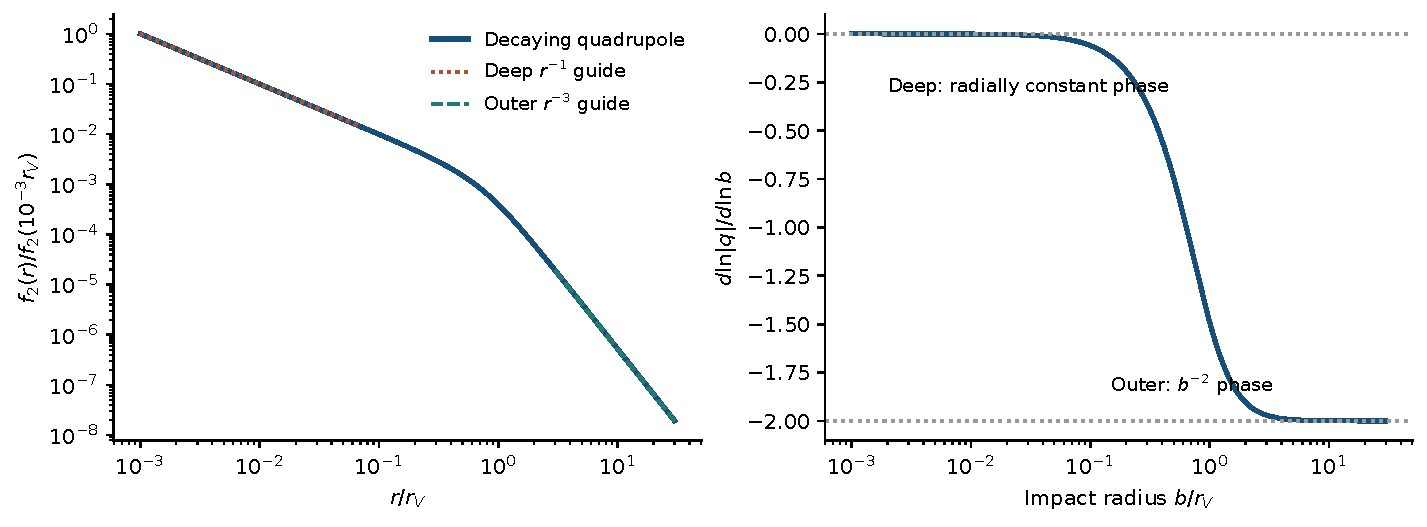
\includegraphics[width=\linewidth]{../figures/screened_transfer.pdf}
\caption{Conditional exterior transfer for the supplied regular-body flux
proxy. Left: normalized decaying quadrupole, with its known deep $r^{-1}$
and outer $r^{-3}$ powers. Right: the slope of the fully matched projected
phase, approaching zero and $-2$. The curves use the action-fixed
coefficients and the full line integral, not an extrapolation of either
power law across the transition.}
\label{fig:transfer}
\end{figure}

\section{Projection and the information retained by the tracker}
\label{sec:projection-information}

The screened multipole exponents and hypergeometric radial modes have cubic-Galileon precedents \cite{Chu2013,Brito2014,Kobayashi2026}. Here the input is the normalized exterior response of the preceding section, with its fixed scalar-to-metric coefficient. The statements below concern that conditional response, rather than a horizon-selected amplitude.

\subsection{A normalized STF boundary state and its projected nulls}

Let $\mathsf C$ be a real symmetric trace-free $3\times3$ matrix, normalized by $\operatorname{tr}\mathsf C^2=1$, and define
\begin{equation}
 Y_{\mathsf C}(\mathbf n)=N_{\rm STF} C_{ij}n_i n_j,
 \qquad N_{\rm STF}=\sqrt{\frac{15}{8\pi}},\qquad
 \int_{S^2}Y_{\mathsf C}^2\,d\Omega=1.
\end{equation}
Thus $a f_2(r)Y_{\mathsf C}$ has boundary $L^2$ norm $|a|$ at $r_0$.
For $\mathsf C_+=\operatorname{diag}(1,-1,0)/\sqrt2$, this is precisely
the transverse harmonic with $N_2=\sqrt{15/(16\pi)}$ used above;
$N_{\rm STF}/\sqrt2=N_2$. Define $\mathcal W=\Phi+\Psi$.
Its scalar-driven response is $\delta\mathcal W=\mathcal A_W f_2Y_{\mathsf C}$,
with $\mathcal A_W=-\widehat\beta a$ for $\pi_T/M_{\rm Pl}$ normalization.
This is the fixed action coefficient, not an additional photon coupling.

For a frozen straight ray with $\mathbf x=(b\cos\varphi,b\sin\varphi,z)$, $b\ge r_0$, factor out $N_{\rm STF}\mathcal A_W$ and the known geometric prefactor. The remaining full-line projection is
\begin{equation}
 \mathcal P_f[\mathsf C](b,\varphi)
 =\int_{-\infty}^{\infty} f(r)\frac{C_{ij}x_i x_j}{r^2}\,dz,
 \qquad r^2=b^2+z^2.
\end{equation}
Parameterize the five STF components by
\begin{equation}
 \mathsf C=\begin{pmatrix}
 -c/2+s_1&s_2&u\\ s_2&-c/2-s_1&v\\ u&v&c
 \end{pmatrix},\qquad
 \operatorname{tr}\mathsf C^2=\frac32c^2+2(s_1^2+s_2^2+u^2+v^2).
\end{equation}
Direct integration gives
\begin{align}
 \mathcal P_f[\mathsf C]&=cA_0(b)
 +T(b)(s_1\cos2\varphi+s_2\sin2\varphi),\label{eq:stf-projection}\\
 T(b)&=b^2\int_{-\infty}^{\infty}\frac{f(r)}{r^2}\,dz,\qquad
 A_0(b)=\int_{-\infty}^{\infty}f(r)
 \left(1-\frac{3b^2}{2r^2}\right)dz.\label{eq:radial-projections}
\end{align}
The $xz$ and $yz$ terms are odd in $z$ and vanish. This exact two-dimensional kernel prevents reconstruction of an unrestricted three-dimensional STF state from this one-view projection. If its three visible coefficients are inferred with the stated action normalization, they only imply
\begin{equation}
 a^2\ge\frac32(ac)^2+2[(as_1)^2+(as_2)^2].
\end{equation}

\paragraph{Conditional rank-three result.}
For the isolated cubic response with
\begin{equation}
 K_r=C_0\sqrt{1+(r_V/r)^3},\quad
 K_\Omega=K_r+\frac r2K_r',\quad C_0>0,\quad r_V>0,
\end{equation}
the normalized positive decaying solution obeys $T(b)>0$ and $A_0(b)>0$. Hence \eqref{eq:stf-projection} has rank three as a map into projected functions, with kernel exactly $(u,v)$. To prove the axial assertion, put $Y=r^3f$. The radial equation implies
\begin{equation}
 (K_r r^{-4}Y')'=6K_r'r^{-5}Y.
\end{equation}
Positivity of $f$ follows from the elliptic maximum principle. Since $K_r'<0$ and $K_r r^{-4}Y'\to0$ at infinity, integration from $r$ to infinity gives $Y'>0$. An integration by parts, using $zf(r)\to0$, then gives
\begin{equation}
 A_0(b)=\frac12\int_{-\infty}^{\infty}\frac{z^2}{r^2}
 [rf'(r)+3f(r)]\,dz
 =\frac12\int_{-\infty}^{\infty}\frac{z^2}{r^4}Y'(r)\,dz>0.
\end{equation}
The genuinely screened hypothesis matters: for $f=C_o/r^3$, $A_0\equiv0$ and $T=4C_o/(3b^2)$, so the rank is two. This harmonic limit agrees with the transverse STF mass-multipole projection \cite{Turyshev2022}. Rank in a projected representation does not by itself establish rank in lens data after monopole and source freedoms are fitted.

These full-line statements use the isolated frozen exterior as a local matching model. Finite observer/source endpoints, nonconstant geometric weights, motion during ray crossing, and cosmological outer completion require their own projection. They cannot be assumed to remove the nulls without calculation.

\subsection{Radial discrimination and its limitation}

In a screened overlap $r_0\le b\ll r_V$, the matched $f\sim A_d/r$ gives
\begin{equation}
 T(b)\sim2A_d.
\end{equation}
The leading transverse potential is therefore constant in radius and spin two in angle. The deep axial integral, temporarily cut off at a symmetric $Z$, is
\begin{equation}
 A_0(b;Z)=A_d\left[2\operatorname{asinh}(Z/b)
 -\frac{3Z}{\sqrt{Z^2+b^2}}\right]
 \sim A_d[2\ln(2Z/b)-3].
\end{equation}
Outer matching fixes the constant and subleading corrections. The leading $-2A_d\ln b$ is degenerate with a point-mass potential. Its additive constant has no deflection or differential-delay signal. The numerical calculation uses the matched profile rather than extending $r^{-1}$ to infinity.

At the potential level, a constant spin-two coefficient differs from an isolated compact harmonic quadrupole proportional to $b^{-2}$ and a uniform external shear proportional to $b^2$. If a calibrated spin-two potential amplitude is restricted to
\begin{equation}
 p_2(b)=q+\mu b^{-2}+\gamma b^2,\qquad D=b\partial_b,
\end{equation}
then
\begin{equation}
 (D^2-4)p_2=-4q.
\end{equation}
At three distinct positive radii, writing $x_i=b_i^2$, the design rows $(1,x_i^{-1},x_i)$ have determinant
\begin{equation}
 -\frac{(x_2-x_1)(x_3-x_1)(x_3-x_2)}{x_1x_2x_3}\ne0.
\end{equation}
Two radii cannot separate $q$ from both nuisance coefficients. For the actual transfer the first column is $T(b_i)$, and its determinant and conditioning must be evaluated. These are conditional potential-reconstruction statements. They are not a claim that three image radii directly measure three potential values. Internal/external multipole reconstruction already has an extensive lensing literature \cite{Trotter2000,Bernstein2009}.

An arbitrary extended matter distribution is a stronger nuisance family: $\nabla_\perp^2[q\cos2\varphi]=-4q\cos2\varphi/b^2$, so an annular distributed quadrupolar density can reproduce this potential. A small quadrupolar perturbation can be supported by a positive monopole. Consequently the radial filter does not identify a gravity theory or exclude an ordinary extended envelope.

\subsection{Timing blindness, scalar-estimator degeneracy, and image geometry}

Use dimensionless reference potential $\psi_0=\ln r$, source $\mathbf y=u\mathbf e$, $s=\sqrt{u^2+4}$ and primary images $\mathbf x_+=a\mathbf e$, $\mathbf x_-=-d\mathbf e$, where $a=(u+s)/2$, $d=a^{-1}$. For a perturbation $q\cos2(\varphi-\varphi_q)$ constant in radius, both unperturbed image potentials agree. Fermat stationarity therefore gives zero first-order delay change at fixed source. Its log flux-ratio change is
\begin{equation}
 \delta\ln R=-4q\cos2(\varphi_s-\varphi_q)\frac{s}{u}.
\end{equation}
Tangential image displacements can retain the angular component absent from this scalar correction. These statements concern continued nonsingular primary branches, with perturbations small enough to avoid a critical crossing or flux-order reversal.

The first-variation operator of the point-lens apparent-mass estimator satisfies
\begin{equation}
 \mathcal K_{1}(u)=\mathcal K_{r^2}(u)
 =\frac{s^3}{u h(u)},\qquad
 h(u)=\frac12us+2\operatorname{asinh}(u/2).
\end{equation}
Thus $(r^2-1)\cos2\varphi$ is an exact first-order null of this scalar statistic for every $u>0$. A deep constant spin-two response and external shear cannot be separated by that statistic alone. The point-lens delay/flux relation is established prior art \cite{Munoz2016}; the evaluated transfer response, rather than different radial powers by themselves, determines its information.
The unit $r^2\cos2\varphi$ profile here has coefficient one in the
potential. In the product's shear convention
$\psi_{\rm shear}=\gamma_+r^2\cos2\varphi/2$, it corresponds to
$\gamma_+=2$. The identity concerns a first variation of this scalar
statistic, not an equality of finite perturbed lens models. The leading
delay null likewise assumes the stated point-lens reference and fixed
source; finite matching corrections to the constant radial profile can
lift it.

\paragraph{Fixed-data gradient proposition.}
Let observed image positions $\boldsymbol\theta_\pm$ and reference Jacobians $A_\pm$ be fixed, and hold the time-delay prefactor fixed. A perturbing potential $p$ can preserve these positions with one freely shifted source if and only if
\begin{equation}
 \nabla p(\boldsymbol\theta_+)=\nabla p(\boldsymbol\theta_-)
 =-\delta\boldsymbol\beta.\label{eq:pair-gradient-null}
\end{equation}
Under \eqref{eq:pair-gradient-null}, the remaining first-order null tests are
\begin{align}
 \delta\Delta\tau&=(\boldsymbol\theta_+-\boldsymbol\theta_-)
 \cdot\delta\boldsymbol\beta+p_+-p_-,\\
 \delta\ln R&=\operatorname{tr}(A_+^{-1}H p_+)
 -\operatorname{tr}(A_-^{-1}H p_-).
\end{align}
The lens equations and Fermat stationarity prove these identities directly. In a forward calculation at fixed source, the images move and the flux derivative also includes the displaced background Hessian; that term cannot be dropped.

For the scalar-estimator null $p=(r^2-1)\cos2\varphi$, direct differentiation gives
\begin{equation}
 \nabla p(a\mathbf e)-\nabla p(-d\mathbf e)
 =2s\cos2\varphi_s\,\mathbf e.
\end{equation}
With a calibrated center, a free source alone cannot absorb this difference when $\cos2\varphi_s\ne0$. An added mass perturbation $\delta m\ln r$ cancels it only for $\delta m=-2\cos2\varphi_s$, which then changes the mass estimator by $\delta m$. Thus image geometry and the estimator distinguish this particular difference if mass is the only additional compensator and the time-distance conversion is fixed. Equivalently, the geometric angular-mass product of the two radii changes by zero for constant spin two and by $2\cos2\varphi_s$ for $r^2$ spin two. Comparing angular and physical masses requires distance calibration.

For $\cos2\varphi_s=0$, the same difference is a genuine first-order joint null for a single freely positioned source: its gradients agree, its source shift is tangential, and both delay and flux-ratio variations vanish. Additional epochs with changing angle can change this rank. Moving centers, convergence, distance factors, ordinary multipoles, and calibration parameters must be included before profiling the full data Jacobian. More general source-position and multi-plane transformations impose further limits \cite{SchneiderSluse2014,Schneider1997,Schneider2019,Fleury2021}. No unrestricted reconstruction theorem follows from the potential-space filter.


\subsection{Incoming, local and outgoing optical transfer}

We use the homogeneous closed R1 background for the incoming and outgoing
distances. If $K=0.018$ in units $L_0=c/H_0$, define
\begin{equation}
 \chi(z)=\int_0^z\frac{dz'}{\widehat H(z')},\qquad
 S_K(\chi)=\frac{\sin(\sqrt K\chi)}{\sqrt K},\quad
 D_{ab}=\frac{L_0 S_K(\chi_b-\chi_a)}{1+z_b}.
\end{equation}
The local deflection then enters the usual single-plane composition,
\begin{equation}
 \boldsymbol\beta=\boldsymbol\theta-
 \frac{D_{ls}}{D_s}\widehat{\boldsymbol\alpha}
       (D_l(\boldsymbol\theta-\boldsymbol c)),\qquad
 \widehat{\boldsymbol\alpha}=\nabla_b\int(\Phi+\Psi)\,dz .
\label{eq:lens-composition}
\end{equation}
This is the homogeneous limit of general optical transfer, whose
equivalent-lens and source-transformation freedoms must be retained
\cite{Schneider1997,Fleury2021,Schneider2019}. No angular environmental
harmonic from the earlier cosmological paper is added here: a second
nonlinear scalar Hessian background would change the local response
operator and require a new reduction.

For a reference mass $M$, let $m=GM/c^2$,
\begin{equation}
 r_E^2=4m\frac{D_lD_{ls}}{D_s},\qquad
 \boldsymbol x=\frac{D_l(\boldsymbol\theta-\boldsymbol c)}{r_E},\qquad
 t_M=\frac{4m}{c}(1+z_l).
\end{equation}
The dimensionless lens potential is the projected Weyl phase divided by
$4m$. In particular, the ordinary monopole is $\ln r$, $r=|x|$; the
scalar monopole correction is derived from the same action. It is added
to that GR metric once. If $q(b)$ is the phase in physical length per
unit transverse boundary amplitude,
\begin{equation}
 \delta\psi=\epsilon_+ Q(r)\cos2\varphi+
                   \epsilon_\times Q(r)\sin2\varphi,
 \quad Q(r)=\frac{q(r_Er)}{q(r_E)},\quad
 \epsilon_A=\frac{a_A q(r_E)}{4m}.
\label{eq:optical-normalization}
\end{equation}
The $a_A$ are supplied scalar states, not extra optical couplings.
Homogeneous metric quadrupoles, which need not be fixed by $a_A$, are
retained as ordinary compact-lens nuisance parameters.

\section{A tracker statistic and its blind direction}

For a point source lensed by an isolated point mass, let $R>1$ be the
absolute primary-image flux ratio. The familiar delay law
\cite{Munoz2016} gives
\begin{align}
 u&=2\sinh(\ln R/4),&s&=\sqrt{u^2+4},\notag\\
 h(u)&=\tfrac12us+2\asinh(u/2),&
 M_{\rm app}&=\frac{c^3\Delta t}{4G(1+z_l)h(u)}.
\label{eq:massstat}
\end{align}
The apparent mass is constant for any slow constant-mass point-lens
trajectory, including source or observer motion incorporated in $u$.
This baseline estimator is inherited. It also remains equal to the point
mass in a constant isotropic convergence in the ideal point-lens model:
rescaling the image/source coordinates leaves the dimensionless
point-mass delay difference and flux relation intact. It is not a general
observable invariant for arbitrary lenses.

For a small additional potential $\epsilon p$, Appendix~\ref{app:estimator-variation}
derives
\begin{equation}
 \delta\ln M_{\rm app}=\frac{\delta\Delta\tau}{h(u)}
          -\frac{s^2}{4h(u)}\delta\ln R.
\end{equation}
Image displacements must enter the magnification derivative even though
Fermat stationarity removes them from the first-order delay at fixed
source. For $p=q(r)\cos2\varphi$, write its response as
$\delta\ln M_{\rm app}=\mathcal K_q(u)\cos2\varphi_s$. An exact
first-order identity is
\begin{equation}
 \mathcal K_1=\mathcal K_{r^2}=K_*(u),\qquad
 \mathcal K_{r^{-2}}=(u^2+1)K_*(u),\qquad
 K_* =\frac{(u^2+4)^{3/2}}{u h(u)}.
\label{eq:blind}
\end{equation}
Thus $(r^2-1)\cos2\varphi$ is invisible to this statistic at first
order for every $u>0$. The potentials differ, and their images, fluxes and
delays generally differ. The cancellation occurs only after compressing
those data into $M_{\rm app}$. In particular, a leading screened
$\epsilon\cos2\varphi$ produces the same apparent-mass history as a
conventional shear $\gamma=2\epsilon$ of the same orientation.
Different radial phase powers alone do not establish identification.

For the radially constant phase, the two primary-image angles differ by
$\pi$, so $p(x_+)=p(x_-)$ and $\delta\Delta\tau=0$. Nevertheless
$\delta\ln R=-4\epsilon s\cos2\varphi_s/u$, and tangential astrometry
can also change. At $\cos2\varphi_s=0$ even the flux/mass statistic is
blind at first order while tangential shifts remain possible. Full
transition matching restores a small radial and delay response
(Figure~\ref{fig:blind}); this does not make the leading degeneracy
irrelevant.

\begin{figure}[t]
\centering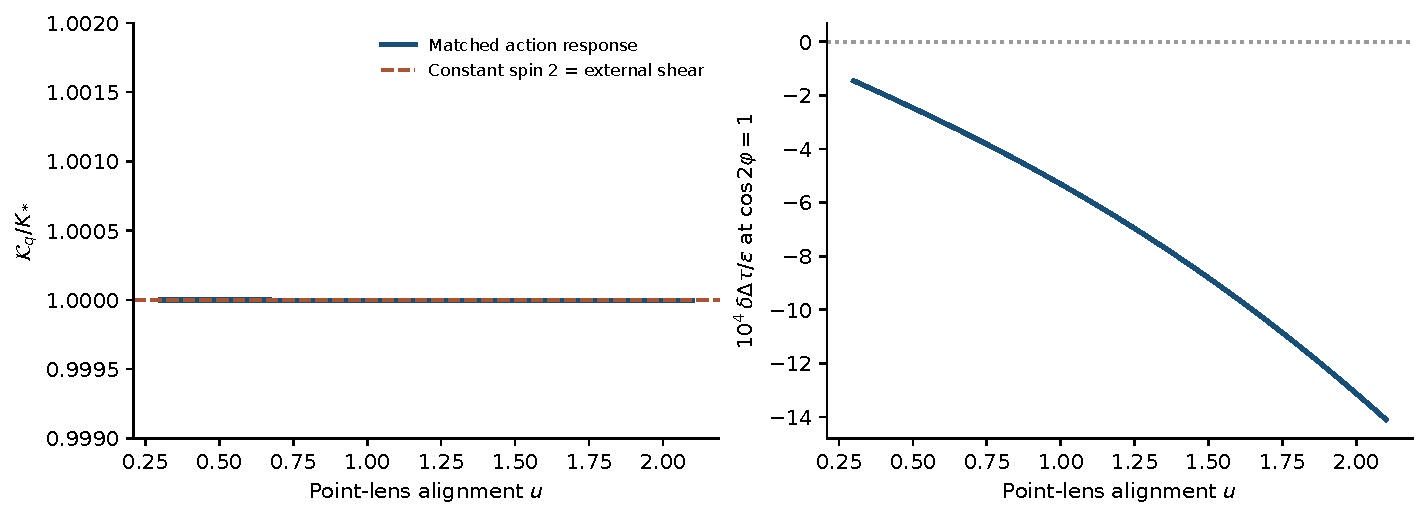
\includegraphics[width=\linewidth]{../figures/tracker_blind_direction.pdf}
\caption{The matched radial profile in the point-mass first-variation
operator, with $r_E/r_V=0.00743$. Left: its apparent-mass response is close
to the exactly coincident constant-phase/external-shear response, despite
different potentials. Right: the small matching-induced delay derivative;
the strict constant-phase result is zero. Curves are derivatives per
dimensionless phase amplitude, not physical observed signals.}
\label{fig:blind}
\end{figure}

\section{Joint primary-pair information experiment}
\label{sec:experiment}

\subsection{Declared data and nuisance family}

The numerical experiment uses the action-derived scalar monopole as well
as the quadrupole, rather than fitting a point-mass background to an
unlabeled modified profile. Its observables at each of nine reference
configurations are
\begin{equation}
 O_i=(x_{+,i},y_{+,i},x_{-,i},y_{-,i},\ln R_i,\Delta t_i/t_M).
\end{equation}
The source reference positions are $(1.8t_i,0.6)$, with $t_i$ uniformly
spanning $[-1,1]$. In the fit, two source coordinates are \emph{free at
every configuration}; no known unlensed track is supplied. They can
absorb parallax, source motion and source-position errors at these sample
points. The lens nuisances are one mass, two center coordinates, two
constant-velocity coordinates, one convergence, two external-shear and
two compact material-quadrupole coordinates. The scalar flux is also
fitted through its local monopole response, rather than assumed known in
the inference. The visible axial scalar quadrupole is also fitted as a
radial nuisance with its normalized $Y_{20}$ response. There are 30 nuisance
parameters and two transverse envelope coordinates in 54 data components.
The two odd projected tensor modes are absent from this one-view data
model rather than artificially fixed by a prior.

The ordinary quadrupoles are $B_A r^{-2}$ and $\Gamma_A r^2$ in the
cosine/sine basis. They are fixed as a family before inspecting the
envelope projection. Internal and external radial multipole information
is familiar in lens modeling \cite{Bernstein2009}; it is not supplied
here as a new general principle. The inference assumes known redshifts,
distances, time calibration and a common absolute astrometric frame.
Unknown frame drift is equivalent to part of the freely fitted center
motion; arbitrary frame distortion or an unrestricted radial potential
is not covered. Fluxes are intrinsic geometric point-source fluxes with
no extinction, blending, independent microlensing or finite-source
structure. These are strong experimental assumptions, not observational
facts.

For each baseline image, $A=I-D^2\psi_0$. The computed response includes
\begin{equation}
 \delta x=A^{-1}(\nabla\delta\psi+\delta y),\qquad
 \delta\ln|\mu|=\tr\!\left[A^{-1}
      (D^2\delta\psi+D(D^2\psi_0)[\delta x])\right].
\label{eq:generalresponse}
\end{equation}
For a translated center, $\delta\psi=-\delta c\cdot\nabla\psi_0$.
Mass differentiation changes the action's scalar monopole too. Source
variation enters the delay as
$(x_+-x_-)\cdot\delta y$, in addition to the potential difference.
These terms ensure comparison of consistent physical states and prevent
spurious source/center signatures.

Let $N$ and $S$ denote the nuisance and envelope derivative matrices.
With a specified data covariance $C_O$, local information is the Gram
matrix of
\begin{equation}
 S_\perp=(I-P_N)C_O^{-1/2}S,
\end{equation}
where $P_N$ projects onto the column space of $C_O^{-1/2}N$.
This is ordinary profiled linear inference. Here all data components
have equal \emph{dimensionless} errors in the displayed units, an
explicit choice for information comparison. It is not an instrument
noise model. Nuisance columns are normalized before SVD; the recorded
rank threshold is $10^{-9}$ of the largest singular value, and the full
spectra are released. Raw column norms below $10^{-11}$ times the larger
of the maximum norm and unity are discarded as numerical zeros.
All 30 full-pair columns survive that admission. The axial mode is nearly
masslike; when all admitted columns have full rank but condition number
exceeds $10^6$, the projection uses 70-digit normal equations after the
unchanged SVD rank selection. An independent 70-digit QR solve checks
the result. These refine arithmetic for the same double-input derivatives,
not the physical approximation. Parameter priors are not added to fill nulls.

\subsection{Evaluated response and controls}

For $M=10^9M_\odot$, $z_l=0.3$, $z_s=1$, $r_0=10$ pc and scalar
flux proxy equal to the regular-body value, the same-background
distances give $r_E=339.62$ pc, $\theta_E=74.116$ mas and
$t_M=25612.55$ s. The computed screening radius is $r_V=45680.31$ pc.
This scale is action-derived after choosing the matching flux; it is not
tuned to the rays.

\begin{table}[t]
\centering\small
\caption{Declared conditional example and local information result. The last
two rows use the small supplied state at source $(0.9,0.6)$; the singular
values use unit optical phase amplitudes and the stated dimensionless data metric.}
\begin{tabular}{p{.49\linewidth}p{.42\linewidth}}
\toprule Quantity & Value\\\midrule
Mass & $10^9M_\odot$\\
Worldtube / Einstein radius & 10.0 / 339.62 pc\\
Screening radius & 45.68031 kpc\\
Worldtube compactness & $4.79\times10^{-6}$\\
Boundary amplitude / optical amplitude & $1.38\times10^{-16}$ / $-8.89\times10^{-13}$\\
Joint-pair nuisance rank & 30\\
Projected envelope singular values & 3.13473, 0.80220\\
Retained column-norm fractions & 0.04213, 0.14512\\
Largest tested physical coordinate shift & $9.36\times10^{-5}$ nanoarcsec\\
Tested physical log-flux-ratio shift & $2.88\times10^{-12}$\\
\bottomrule\end{tabular}\label{tab:numeric}\end{table}


The joint-pair projected envelope singular values are approximately
$(3.135,0.802)$ per unit phase amplitude. Roughly 4--15\% of each
envelope column's norm survives the 30 nuisance directions. The strict
constant-phase replacement gives nearly the same joint-pair result;
identification here therefore comes mainly from keeping the separate
image/flux/delay information rather than resolving the small transition
correction. Astrometry alone retains only very small directions in this
example, and its near-null spectrum is numerically delicate. The
apparent-mass statistic alone retains no measurable independent
direction with the admitted free-source/action-monopole family. The
analytic point-mass/shear null in Equation~\eqref{eq:blind} separately
establishes an exact first-order loss without relying on an SVD cutoff.

\begin{figure}[t]
\centering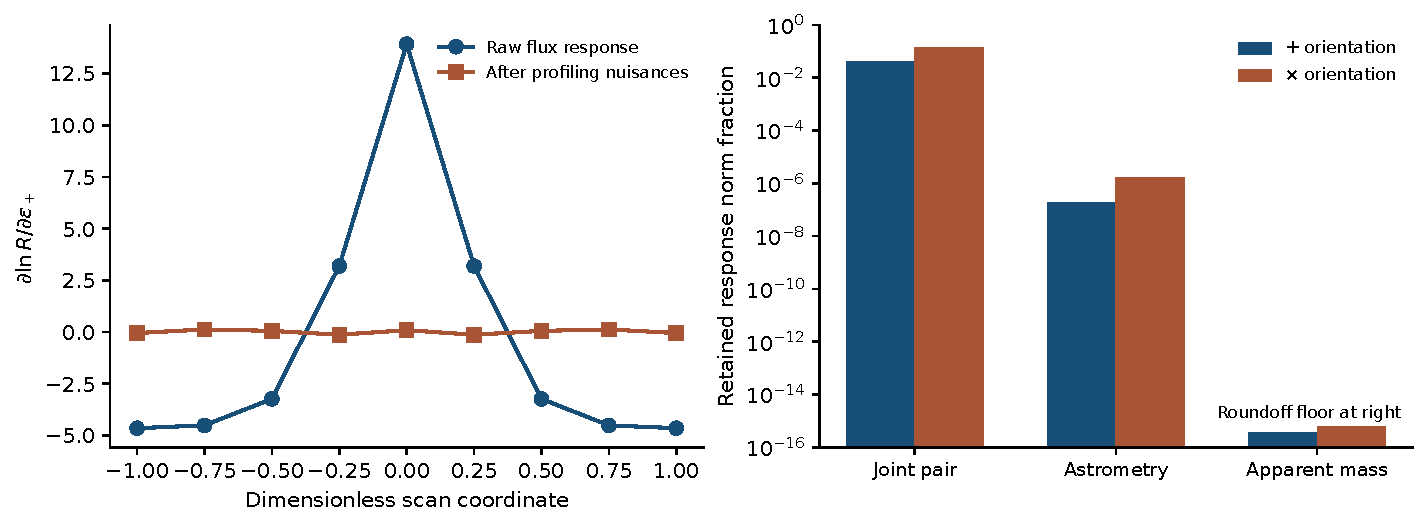
\includegraphics[width=\linewidth]{../figures/tracker_information.pdf}
\caption{Information retained by the declared broad scan. Left: the flux
component of the $+$ response before and after simultaneous nuisance
projection in the full data vector. Right: retained column-norm fractions
for three data choices; the apparent-mass residual is at roundoff.
Comparisons use the stated dimensionless metric and nuisance family,
not a telescope covariance or a universal observability theorem.}
\label{fig:information}
\end{figure}

Controls vary mass, worldtube radius and the supplied scalar flux. With
zero spherical scalar flux the exterior quadrupole is harmonic,
$f_2\propto r^{-3}$; its transverse projected phase is exactly an ordinary
compact quadrupole and the retained response vanishes to numerical
precision. Nonzero fluxes $0.1$, $1$ and $3$ times the proxy give a
screened response with the same broad-scan information pattern, as do
the tested $10^6$ and $10^{11}M_\odot$ examples with declared weak-field
worldtubes. These are conditional boundary families, not alternative
theories or inferred black-hole charges. Allowing an independent center
at every configuration reduces the joint information but does not remove
both transverse directions in this restricted family. Arbitrary
time-dependent quadrupoles would be a different, less constrained problem.

\subsection{Perturbative and numerical control}

The physical state example is chosen by an explicit small parameter,
\begin{equation}
 a_+=\frac{\eta x_0|p(x_0)|}{6},\quad a_\times=0,
 \qquad \eta=10^{-3},\quad x_0=r_0/L_0.
\label{eq:smallstate}
\end{equation}
The factor six is the quadrupole angular eigenvalue; the numerical
checks also evaluate actual Hessian ratios and the quadratic residual
in the retained nonlinear scalar equation. This is a supplied
perturbatively small state, not a BHSM-selected amplitude or an upper
bound on astrophysical deformations. It gives $a_+\simeq1.38\times10^{-16}$
and $\epsilon_+\simeq-8.89\times10^{-13}$.

At source $(0.9,0.6)$ the retained model gives a largest coordinate shift
of about $9.4\times10^{-5}$ nanoarcsec and
$\delta\ln R\simeq2.88\times10^{-12}$. The formal matched delay
shift is approximately $5.1\times10^{-12}$ s. That last small number
is a value in the truncated static thin-lens model, whose leading delay
term vanishes; it is \emph{not} a physically certified picosecond forecast.
Uncomputed time-dependent and matching corrections require their own
comparison before interpreting such a subleading delay.

The code checks the radial equation against the special-function
solution, the dipole translation mode, independent original-$z$ versus
transformed line integrals, finite-difference projected derivatives,
boundary energy normalization, and finite nonlinear primary-image
continuations. At test amplitudes decreasing from $10^{-3}$ to
$3\times10^{-5}$, the central-difference error in the full response
decreases quadratically to about $1.6\times10^{-7}$, with image
stationarity residuals below $10^{-14}$. Those larger optical test
amplitudes test the lens derivative; they do not validate the small-state
scalar linearization at an enlarged boundary amplitude. Independent
symbolic/Cartesian and polynomial-branch checks verify the estimator
operator and its nulls. All are internal AI-assisted checks.

Quintic interpolation uses analytic projected derivatives at logarithmic
nodes; measured midpoint discrepancies and quadrature refinements are
recorded as numerical diagnostics, not interval certificates. The formal
infinite exterior is matched to the frozen local background. At a
1 Mpc cutoff, explicit far-tail bounds give a monopole deflection tail
below $9\times10^{-11}$ of the ordinary deflection and a transverse
quadrupole phase tail below $8\times10^{-11}$ pc per unit boundary
amplitude. These bound omitted tails only. They do not bound every
weak-field, cosmological or effective-theory correction.

\section{Materials and methods: the runnable Blackhole Tracker product}
\label{sec:product}

The released research product makes the compact-lens measurement task
operational. A local browser app, command line, importable Python package
and four executed notebooks provide separate versioned resolved-pair,
native-photometry and joint astrometry/parallax contracts. This is an offline analysis tool; the
resolved mode described here takes supplied primary-pair measurements.
The native route and its measured-data pilot are treated in
Section~\ref{sec:real-observations}. Its
ordinary-lens mode estimates the mass, center and motion of the
BHSM-described exterior, with the explicit boundary dictionary of
Section~\ref{sec:bhsm-interpretation}. Its optional R1 mode evaluates the
conditional exterior and the admission bound of
Section~\ref{sec:admission-bound}. Established lens software already
supports sophisticated lens inference: \texttt{lensmodel},
\texttt{lenstronomy} and \texttt{PyAutoLens}
\cite{Keeton2001,Birrer2018,Nightingale2021}; the moving-lens
\texttt{BAGLE} framework is a particularly close predecessor
\cite{Lu2025}. No first mass/motion tracker or general replacement for
those tools is claimed.

The comparison is specific. Cubic-Galileon multipole calculations
\cite{Chu2013,Brito2014} supply screening powers and Green functions;
general STF lens projection \cite{Turyshev2022} supplies multipole
transfer methods. Here those ingredients are composed with the adopted
R1 coefficients, a normalized boundary/conormal pairing and a sufficient
state cap, followed by explicit delay/statistic nulls. The extended-source
lens packages above address broader image reconstruction and lens
inference; \texttt{BAGLE} models moving microlenses with astrometric,
photometric and parallax information. This product instead takes
resolved primary pairs, their geometric flux ratio, supplied delays and
a full covariance, and reports the conditional BHSM dictionary and R1
admission/information assessment. It supplies no general extended-image
reconstruction, survey acquisition or observational validation of those
assumptions. No superiority or priority follows from these scope differences.

\paragraph{Computational methods and generative AI.}
The reproducible software is Blackhole Tracker, version 0.2.0rc4;
the versioned source, environments and executable checks are supplied
with the release. OpenAI ChatGPT and Codex (GPT-6 model family) assisted
source recovery, mathematical derivation, code and test generation,
numerical analysis, literature checking and manuscript drafting.
Synthetic measurements are generated by the released numerical model,
not by language-model sampling. Symbolic identities, finite differences,
numerical residuals, source hashes and independent internal agent checks
test the retained output. These checks do not replace author review or
external peer review; their scope and limitations are reported below.

\subsection{Measurement contract and likelihood}
An input supplies angular-diameter distances $D_l,D_s,D_{ls}$, redshifts,
a reference observer epoch, and $N$ epoch/source rows, with $3\le N\le80$.
Each row contains two resolved image positions in mas,
$\ln(|\mu_+|/|\mu_-|)$ and the negative-parity minus positive-parity
arrival-time difference in seconds. The labels refer to parity, not a
brightness ordering; a perturbed flux ratio may be below unity.
The covariance is the full positive-definite $6N\times6N$ matrix in
row-major observable order. Neither time sorting nor diagonalization is
applied. Correlated astrometric, flux and timing errors therefore remain
coupled under Cholesky whitening. A provenance field explicitly declares
synthetic or observed measurements. Validation of that field and the
numerical schema does not verify an observation's origin.

With supplied parallax factors $\boldsymbol P_i$, the lens center is
\begin{equation}
 \boldsymbol c_i=\boldsymbol c_0+
 \boldsymbol\mu_{\rm obs}(t_i-t_0)
 +\frac{1000}{D_l/\mathrm{pc}}\boldsymbol P_i\;\mathrm{mas}.
 \label{eq:product-track}
\end{equation}
Omitting these factors means a declared zero observer-parallax term.
Distances, the astrometric frame and timing calibration are treated as
known; they are not silently inferred from the lens data. The source
position has two free coordinates at every row, even when several rows
represent repeated observations of one source. Source trajectory truth
is never supplied to the fitter. The ordinary model contains a point
mass and constant center motion, with selectable shear or the larger
family of shear, convergence and compact quadrupole. It solves the
nonlinear lens equation for the continued positive/negative primary
branches, rejects critical or incorrectly ordered branches, and uses
their full magnification determinants and Fermat delay.

The optimizer minimizes
\begin{equation}
 \chi^2(\vartheta)=\|L^{-1}[d-f(\vartheta)]\|_2^2,
 \qquad LL^T=C.
 \label{eq:product-likelihood}
\end{equation}
An analytic point-lens delay/flux initializer supplies a computational
mass scale, followed by deterministic perturbed starts and bounded
nonlinear least squares. The default mass search domain is
$[10^{-3},10^{12}]M_\odot$, exposed in the input rather than confused
with a detection prior. A conservative slow-motion domain is declared
separately. Final solutions undergo primary-branch, actual-impact
weak-field and motion checks; R1 additionally requires its exterior
worldtube and state-admission conditions. Local covariance follows the whitened Jacobian SVD,
without rescaling the supplied $C$ by reduced $\chi^2$. Null directions
have unavailable uncertainties. Center-track bands propagate the
center--motion cross covariance. Reoptimized one-coordinate likelihood
profiles are available from the command line and notebook; their usual
$\Delta\chi^2$ reference values do not guarantee nonregular coverage.

The reviewed implementation optimizes near a data-derived epoch without
finite numerical boxes on center or source positions. It reports the
center at the supplied epoch using
$\boldsymbol c_{\rm rep}=\boldsymbol c_{\rm opt}+
\boldsymbol\mu(t_{\rm rep}-t_{\rm opt})$.
The full identified-subspace covariance and null directions transform
with the reporting Jacobian, including center--motion cross terms.
Unidentified physical covariance is unavailable; a truncated inverse is
not reported as precise motion uncertainty. Weak but identifiable motion
retains finite covariance. Numerical reference mass changes do not alter
the physical position domain or the separately fixed physical bounds of
compact multipoles. Persisted basis metadata prevent reinterpretation of
legacy internal coordinates.

Each fixed-parameter profile genuinely searches admissible nuisance
states under the public weak-field, worldtube, motion and conditional-R1
constraints. Interior and boundary optima remain distinct from numerical
failure and unresolved physical-domain searches. A failure to find an
admissible state does not prove infeasibility. Only admitted solved rows
relative to an admitted reference minimum can supply a physical
likelihood crossing; unresolved rows have unavailable likelihood values.

\subsection{Product decisions and the conditional extension}
\texttt{FIT\_REJECTED} denotes solver failure, unacceptable residuals
at the declared $p<0.001$ guard, or failure of a physical-domain check.
\texttt{INSUFFICIENT\_INFORMATION} denotes unavailable or very weak mass
information. Otherwise, \texttt{PARTIALLY\_IDENTIFIED} reports weak
motion or a global parameter at its search bound.
\texttt{TRACKED} requires a supported mass and a two-dimensional local
motion Mahalanobis radius of at least five, together with the other
checks. This is a transparent product decision rule within the supplied
model and covariance; it is not a black-hole classification or a
universal false-alarm probability. Every result retains its full
residuals, assumptions and diagnostics.

In R1 mode the spherical flux is either the explicitly labeled fixed
regular-body proxy or a fitted conditional matching datum. The latter
is bounded to the declared fitted domain $0.05\le\chi\le20$; discrete
runtime comparisons do not certify that entire interval. Neither option is called
horizon matched. After fitting the monopole and ordinary nuisances,
unit-amplitude transverse responses are whitened and projected off the
fitted Jacobian and the visible axial response. If their singular
values are $s_1\ge s_2$, the diagnostic compares
$\mathcal A_{\max}s_j$ with unity. A rank loss or best admitted response
below unity returns \texttt{UNRESOLVED}. The alternative label,
\texttt{INFORMATION\_AVAILABLE}, denotes local conditional sensitivity,
not a detected deformation. A formal unconstrained state outside the
cap is explicitly marked outside the admitted family. The product does
not inflate it into a physical fit.

For the noisy nearby fixture below, the ordinary fit gives
$M=99947.2\pm38.7\,M_\odot$ and
$\boldsymbol\mu=(0.06667,-0.03808)$ mas/yr with local component errors
$(0.00119,0.00123)$ mas/yr; $\chi^2=36.39$ for 29 degrees of freedom.
These are one synthetic realization's outputs. For R1 analysis with the
fixed regular-body flux proxy and shear nuisances, that fixture can
retain the ordinary track while returning an unresolved envelope: the
admitted state cap is about $5.34\times10^{-21}$ and the largest
projected admitted local response-to-noise is about
$2.33\times10^{-14}$. Thus making the tracker usable does not supply
evidence for the proposed BHSM deformation signal.

The app supports input inspection, validation, fitting, track and
observable plots, uncertainty/null diagnostics and JSON/HTML export.
Both app and command line export a complete replay analysis: original
input with full covariance and calibrations, fit configuration, installed
software/source hashes, fitted parameters, predictions, diagnostics,
interpretation, plots and a SHA-256 manifest. The command
\texttt{python -m bhtracker replay analysis.zip -{}-output replayed}
verifies hashes and repeats resolved/native-photometry inference. The
resolved/native refit comparison
requires unchanged scientific status and prediction differences below
$10^{-3}$ of each supplied marginal standard deviation; this is not a
rescaling of measurement error or a statistical detection threshold.
For the separately versioned joint route, replay verifies the saved
nonlinear state, profiled nuisances and predictions with its pinned
scientific source. It does not repeat optimization or certify noise
adequacy, mass support or black-hole classification.
The first notebook reproduces
mass/motion inference, a mass profile and the weak-motion control; the
second evaluates conditional response and admission. The third preserves
native unresolved photometry. The fourth verifies the separately versioned
joint likelihood, source-pack import and archived measured-state replay;
its successful execution does not accept the measured benchmark's mass.
Raw theory inputs
are packaged and hash checked, so these interfaces do not depend on a
private archive path or the author's checkout. A separate stellar-mass
example adapts rounded parameters from \citet{Lu2025} into a declared
synthetic primary-pair test with a chosen observer ellipse. Its positions,
fluxes and added delays are generated by this product. No \texttt{BAGLE}
engine was run, and no observed data or real ephemeris was validated.
The independent ordinary-lens checks instead evaluate the analytic
point-mass equations in physical units separately from the package's
lens helpers. The repeated-noise experiment tests recovery and local
interval coverage under the product's own declared synthetic model.

\paragraph{Versioned historical calibration.}
The following resolved-pair calibration retains its original 64-draw
experiment and separate 128-draw follow-up, source versions and failed
controls. It is historical evidence for that model and implementation,
not a repeated calibration of the revised rc3 kernel or native
unresolved-photometry likelihood.
\section{Results: nonlinear product validation with known covariance}
\label{sec:product-validation}
The software product is tested separately from the preceding
54-observable theory experiment. Its ordinary compact-lens inference fits
mass, reference center and observer proper motion, two shear components,
and two free source coordinates at every row. Distances, redshifts and the
absolute astrometric frame are supplied calibrations. The baseline
validation is entirely synthetic; its adopted errors do not specify an
instrument capability. Optional R1 information retains the separate
conditional-exterior and physical-amplitude restrictions.
The frozen nearby fixture contains a $10^5 M_\odot$ lens at $D_l=1$ Mpc,
three background source positions sampled at each of three epochs over
ten observer years, and true motion $(0.065,-0.038)$ mas/yr.
The nine rows supply 54 image-coordinate, log-flux-ratio and delay
measurements. Their declared base noise scales are $0.02$ mas, $0.005$ and
$3\times10^{-4}$ s, respectively, with supplied astrometric and timing
correlations. The full covariance $C$ is retained in
$\chi^2=(d-f)^T C^{-1}(d-f)$; errors are not rescaled by the fitted
reduced $\chi^2$. These inputs test a resolved primary-pair model with
free source positions, rather than assume a known unlensed source track.

\begin{figure}[tbp]
\centering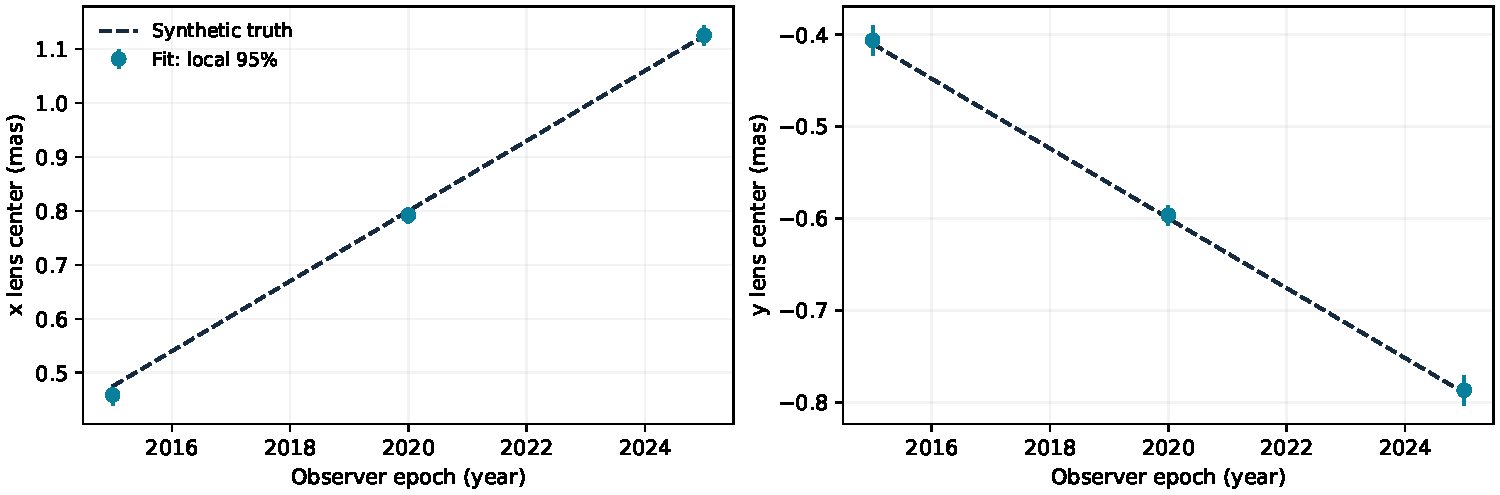
\includegraphics[width=\linewidth]{../figures/product_track.pdf}
\caption{The noisy nearby synthetic fixture: recovered lens-center
coordinates with local 95\% marginal intervals propagated from the full
center--motion covariance, against truth used only for scoring.
Repeated rows at each epoch overlap. This is a ten-year three-source
product test, distinct from the broad single-track information scan.}
\label{fig:product-track}
\end{figure}

The noiseless recovery control (C6) uses the data-derived initializer and
two fixed perturbations, including mass factors 1.5 and 0.65 and shifts
of center, motion, sources and shear. Each fit uses three internal starts.
All recover the mass, center and motion within the frozen relative or
reference-scale tolerances $10^{-5}$; the largest $\chi^2$ is
$3.01\times10^{-23}$, below the fixed $10^{-6}$ criterion. Truth is used
to score recovery, not supplied as an initializer. This checks nonlinear
solver recovery for this fixture, not global likelihood uniqueness.

\subsection{A fixed repeated-noise calibration}
Control C7 draws 64 independent Gaussian noise vectors using the full
$C$, a single frozen PCG64 stream seeded 4932026, and one start per
ordinary-lens fit with shear admitted. Every realization remains in the
record and coverage denominator; an exception, rejected fit or unavailable
interval would count as a miss. All 64 fits converge and return the
product's \texttt{TRACKED} status, with no excluded failures.
The reported intervals are local known-covariance Gaussian intervals,
not reoptimized likelihood profiles. For mass we use
$\widehat M\exp[\pm1.959964\,\sigma_M/\widehat M]$; center and motion
use $\widehat\theta\pm1.959964\,\sigma_\theta$.

\begin{table}[tbp]
\centering\small
\caption{Frozen 64-draw local 95\% interval coverage. Each exact two-sided
binomial test has null coverage 0.95 and rejection level $\alpha=0.01$.
All five tests are reported without a multiple-testing adjustment.}
\label{tab:product-coverage}
\begin{tabular}{@{}lrrr@{}}
\toprule
Coordinate & Covered / 64 & Fraction & Exact $p$\\
\midrule
Mass $M$ & 61 & 0.9531 & 1.0000\\
Center $x$ & 59 & 0.9219 & 0.2532\\
Center $y$ & 61 & 0.9531 & 1.0000\\
Motion $x$ & 61 & 0.9531 & 1.0000\\
Motion $y$ & 61 & 0.9531 & 1.0000\\
\bottomrule
\end{tabular}
\end{table}

None fails the preregistered gross-miscalibration guard
(Table~\ref{tab:product-coverage}). The exact 95\% binomial interval for
61/64 coverage is $[0.8691,0.9902]$, and for 59/64 it is
$[0.8270,0.9741]$: 64 draws provide a limited calibration check.
The receipt also retains parameter bias and scatter. In particular, the
mean $y$-motion error is $3.98\times10^{-4}$ mas/yr, about 2.75 estimated
standard errors of its ensemble mean. Passing the frozen coverage test
does not establish negligible bias or universal coverage.

\subsection{A bounded investigation of the mean offset}
Before generating follow-up data, a separate protocol fixed an independent
analytic linear-noise control, tighter checks of original indices 0--7,
and, conditional on those checks, exactly 128 further draws from PCG64
seed 202610210128. The original receipt, thresholds and 64-draw table are
unchanged; the two ensembles are not pooled. The protocol's initially
announced version was clarified before execution to specify that mean
diagnostics use all finite returned estimates, including those returned
with rejected decisions; such decisions remain interval-coverage misses.
The revision history and both hashes are retained in the risk receipt.

The independent 25-column point-lens, shear and free-source Jacobian uses
stationary-image derivatives in physical units. Its whitened relative
discrepancy from the production Jacobian is $2.50\times10^{-11}$, and the
largest discrepancy of the five covariance diagonals is
$2.91\times10^{-11}$, below fixed bounds $10^{-5}$ and $10^{-4}$.
Its original-sample mean $y$-motion error is
$3.98022\times10^{-4}$ mas/yr, versus the nonlinear
$3.97992\times10^{-4}$ mas/yr: their difference is only
$-0.000199$ analytic standard errors of the ensemble mean.
The offset is therefore already present in a first-order response with
exactly zero expected error. The largest mean nonlinear-minus-linear
discrepancy among all five coordinates is $0.00509$ analytic standard
errors, below the fixed $0.1$ concern level. Eight tighter refinements
change estimates by at most $4.57\times10^{-8}$ local standard deviations
and improve $\chi^2$ by at most $1.55\times10^{-12}$, below the respective
fixed bounds $0.01$ and $10^{-6}$. These checks find no material covariance
or local convergence discrepancy in this fixture.

\begin{table}[!b]
\centering\small
\caption{Separate fixed 128-draw follow-up. Rejected decisions count as
misses. Coverage tests retain null 0.95 and per-coordinate
$\alpha=0.01$. Mean $z$ uses the known truth linear covariance; the
prespecified five-coordinate mean guard has Bonferroni familywise
$\alpha=0.01$.}
\label{tab:product-risk-followup}
\begin{tabular}{@{}lrrr@{}}
\toprule
Coordinate & Covered / 128 & Exact coverage $p$ & Mean $z$\\
\midrule
Mass $M$ & 118 & 0.1513 & $-0.4555$\\
Center $x$ & 120 & 0.5383 & $-0.2571$\\
Center $y$ & 119 & 0.3045 & $-0.1777$\\
Motion $x$ & 120 & 0.5383 & $-0.7367$\\
Motion $y$ & 121 & 0.6872 & $0.8394$\\
\bottomrule
\end{tabular}
\end{table}

All 128 optimizers converge and return finite estimates; 126 decisions
are \texttt{TRACKED} and two are \texttt{FIT\_REJECTED} at the unchanged
goodness-of-fit guard $p<0.001$. All remain in the record and denominator
(Table~\ref{tab:product-risk-followup}). Neither the coverage nor local
mean-error guards reject. The follow-up $y$-motion mean is
$9.13\times10^{-5}$ mas/yr, or $0.879$ empirical ensemble standard errors.
The mean diagnostics include finite estimates from the two rejected
decisions as specified; they are not admitted tracks. A labeled post-hoc
projection of the already-used noise through the independent linear
model rejects exactly the same two draws, with $\chi^2=65.4492,70.3639$
on 29 degrees of freedom, compared with nonlinear $65.4439,70.3620$.
Two such rejections are uncommon under an ideal size-0.001 guard:
$\Pr[\mathrm{Binomial}(128,0.001)\geq2]=0.00748$. This limitation is
retained without changing thresholds or replacing data. The study does
not calibrate an operational false-rejection rate.

The bounded execution uses 145 solves and leaves the reserved correction
stream unused. No production bias correction or recentering is applied.
These results are consistent with finite-sample fluctuation of the
highlighted offset in this fixture, while preserving its observed value.
They support limited synthetic local-interval calibration, not proven
unbiasedness, universal coverage or observational sensitivity.

\subsection{Weak information, model mismatch and finite cause ambiguity}
The negative controls preserve unsuccessful scientific outcomes
(Table~\ref{tab:product-controls}). The ten-year cosmological fixture
(C8) has true motion $(5,-3)\times10^{-5}$ mas/yr and returns
\texttt{PARTIALLY\_IDENTIFIED}, with motion signal-to-noise 0.00482 and
component errors $(0.0121,0.0124)$ mas/yr. Its mass information does not
license a resolved motion claim. For a separate conventional-shear
fixture (C11), omitting shear gives a rejected fit at the frozen
goodness-of-fit criterion $p<0.001$; admitting shear recovers the declared
$(0.03,-0.018)$ coefficients. Residual structure is therefore not assigned
automatically to an R1 envelope or a new physical cause.

\begin{table}[tbp]
\centering\small
\caption{Controls with scientifically meaningful weak or null outcomes.}
\label{tab:product-controls}
\begin{tabular}{@{}lll@{}}
\toprule
Control & Quantity & Outcome\\
\midrule
C8: short cosmological track & Motion SNR $0.00482$ & Unresolved motion\\
C11: shear omitted & $\chi^2=28297.8$ & Fit rejected\\
C11: shear admitted & $\chi^2=1.95\times10^{-22}$ & Baseline recovered\\
C9: harmonic / compact pair & Four columns, rank two & Two exact nulls\\
\bottomrule
\end{tabular}
\end{table}

For C9 the zero-flux harmonic boundary response is exactly an ordinary
compact $r^{-2}$ quadrupole, with coefficient
$-\widehat\beta N_2 r_0^3/[3m_{\rm ref}(r_E^{\rm ref})^2]$ per boundary
amplitude, in the declared reference lens units.
Three finite operator comparisons and compensating coefficient changes
agree in potential, gradient and Hessian to $2.22\times10^{-16}$.
Four combined compact/boundary columns have rank two. Large formal
coefficients are confined to this operator identity test; public
prediction separately rejects that nonadmitted state. They are not
enlarged physical signals. The current nonlinear fit does not expose a
joint free fit of both degenerate amplitude pairs, so separate-amplitude
interval calibration is not claimed.
These controls accompany the released independent interface, physical-unit,
covariance and admission tests. Versioned JSON receipts retain every
draw, initializer, criterion, runtime and SHA-256 source hash; the R1
provider inputs are pinned and checked on loading. The scripts
\texttt{calibrate\_product.py} and
\texttt{check\_finite\_harmonic\_degeneracy.py} reproduce the controls.
The validated scope is the declared synthetic compact-lens families and
local intervals. Unknown calibration, broader environmental freedom,
critical image configurations, observational sensitivity and horizon
identification remain outside this validation.

\subsection{A new frozen validation of the corrected kernel}
\label{sec:current-kernel-calibration}
The preceding calibration receipts remain historical experiments with their
original sources and criteria. A separate prospective study on 24 October
2026 tests the corrected kernel with independently written lens equations
and two authentic cadence/error patterns. All brightnesses and resolved
measurements in this study are synthetic. No resolved image positions,
flux ratios, delays or distances are attributed to an actual event.
The fixed design contains 4\,608 generated datasets, 4\,736 fits and
1\,024 generating-timescale profile queries. Every planned fit is retained;
there are no generation, fit/score or serialization exceptions. A completed
fit can nevertheless be rejected or unidentified. The full accounting,
input lineage, exact binomial intervals, residual plots and source hashes
are supplied with the versioned research protocol.

Four resolved blocks each contain 512 realizations: a $10M_\odot$ lens,
the same physical design with a remote reporting epoch and a changed
numerical mass reference, a $0.05M_\odot$ lens, and a $10^5M_\odot$ lens.
Physical distances, frame and dense Gaussian covariance are supplied
hypothetical calibrations. The twenty local-coverage tests for mass,
center and motion do not reject at the frozen Bonferroni family level
$0.01/28$. This is conditional evidence at the specified designs; it
does not calibrate unknown instruments, actual-object distances or a
black-hole classifier.

\begin{table}[tbp]
\centering\small
\caption{Unconditional local nominal 95\% coverage in the new frozen
study. All denominators are 512, including scientifically rejected fits.
The last column is generating-timescale profile-reference membership,
not a complete confidence interval. Asterisks identify the three
rejections among the fixed family of 28 tests.}
\label{tab:current-kernel-coverage}
\begin{tabular}{@{}lrrrrrr@{}}
\toprule
Resolved design & $M$ & $x$ & $y$ & $\mu_x$ & $\mu_y$ & \\
\midrule
$10M_\odot$ & 485 & 484 & 488 & 488 & 486 & \\
Remote reference & 492 & 494 & 498 & 493 & 499 & \\
$0.05M_\odot$ & 483 & 483 & 481 & 483 & 491 & \\
$10^5M_\odot$ & 490 & 489 & 489 & 490 & 491 & \\
\midrule
Photometric cadence & $t_0$ & $t_E$ & $u_0$ & & & Profile \\
\midrule
OGLE3-ULENS-0033 & 485 & 478 & 475 & & & 478 \\
OGLE3-ULENS-0127 & 482 & $510^{*}$ & $461^{*}$ & & & $504^{*}$ \\
\bottomrule
\end{tabular}
\end{table}

The stationary resolved block returns zero motion detections among 256
realizations at the existing two-component Mahalanobis signal-to-noise
cut of 5. Its exact one-sided 95\% upper rate is about 1.16\%, which does
not verify a conventional one-dimensional five-sigma false-alarm rate.
Both repeated-epoch blocks retain unavailable motion covariance in all
64 realizations. The 128 ordinary-shear inputs are rejected when shear
is omitted and tracked when it is fitted. The low-mass block never crosses
the engineering optical-mass comparator of a lower local bound above
$3M_\odot$; this comparator is not a universal neutron-star limit or a
validated black-hole classification.

The native-magnitude controls preserve the times, errors and row identities
of OGLE3-ULENS-0033 and OGLE3-ULENS-0127, while replacing every brightness
in a separately labeled synthetic daughter. Underlying photometric clocks
remain unspecified. On the second cadence, local $t_E$ intervals cover
510/512 truths (99.61\%) and local $u_0$ intervals cover 461/512 (90.04\%);
the generating-timescale reference set contains truth in 504/512 (98.44\%).
The exact two-sided nominal-0.95 binomial probabilities are respectively
$2.96\times10^{-9}$, $3.78\times10^{-6}$ and $6.54\times10^{-5}$.
All three fail the frozen multiplicity-adjusted criterion. Overcoverage
is reported alongside undercoverage. These findings prevent interpreting
the local errors or the profile-reference threshold as universally
calibrated 95\% confidence statements; the profile query does not measure
finite endpoints or a lens mass.

Goodness-of-fit nonrejection is also insufficient to establish a lensing
origin. Constant-source controls are not rejected in 94/128 and 102/128
cases on the two cadences. The specified periodic-variable controls are
rejected in all cases. The two-source controls are rejected in all 128
cases on the first cadence but are not rejected in 125/128 on the second.
Correlated-noise point-lens controls are not rejected in 121/128 and
112/128 cases. These are fixed-design screening rates, not population
frequencies or black-hole false-positive rates. All 2\,048 photometric
cases retain unavailable mass and distance.

An independent saved-only audit verifies the input/result lineage,
quadratic forms, denominators and all 28 exact tests, without drawing
noise or calling a model, optimizer or profile. It confirms the three
calibration failures. The scientific publication hold remains: no known
black-hole recovery, BH classification error rate or new black-hole
identification follows from this synthetic study. Its BHSM interpretation
is the same single Einstein/GHY optical exterior as gravitational surface
topography, counted once; it measures no microscopic core or horizon.

\section{Native unresolved observations: a frozen 100-event pilot}
\label{sec:real-observations}

\subsection{A separate observation contract and its identifiable quantities}

The resolved-pair experiments above are not the observation model for an
unresolved survey light curve. Release candidate 0.2.0rc3 adds a separate,
versioned native-photometry route. An input row retains its original
time, apparent magnitude, uncertainty, instrument/filter, source file hash
and source-line identity. Catalog coordinates, aliases, calibration notes
and documented warnings remain provenance. No image positions, primary
flux ratios, interimage delays, distances or covariance are manufactured
from those rows.

For a rectilinear point-source point-lens (PSPL) event
\cite{Paczynski1986}, the dimensionless source--lens separation and
unresolved magnification are
\begin{equation}
 u(t)^2=u_0^2+\left(\frac{t-t_0}{t_E}\right)^2,\qquad
 A(u)=\frac{u^2+2}{u\sqrt{u^2+4}}.
 \label{eq:native-pspl}
\end{equation}
For instrument $j$, $F_j=F_{s,j}A+F_{b,j}$. Writing the baseline
magnitude as $m_{b,j}$ and the baseline source fraction as
$f_j=F_{s,j}/(F_{s,j}+F_{b,j})$ gives the native-magnitude prediction
\begin{equation}
 m_j(t)=m_{b,j}-2.5\log_{10}\!\left[1+f_j(A(u(t))-1)\right],\qquad
 \chi^2=\sum_i\frac{[m_i-m_{j(i)}(t_i)]^2}{\sigma_i^2}.
 \label{eq:native-magnitude-likelihood}
\end{equation}
This likelihood assumes independent Gaussian errors in the supplied
native magnitudes. It preserves the supplied errors; it does not infer
an unprovided cross-row covariance or establish that the independence
assumption is correct. Per-instrument baselines absorb independent
photometric zero points without treating published catalog parameters as
new measurements. The catalog solution initializes one of twelve
deterministic starts and contributes no likelihood term.

The optical model has the same BHSM Einstein/GHY interpretation as
Section~\ref{sec:bhsm-interpretation}: one effective exterior acts once.
Unresolved PSPL photometry, however, generally constrains only event
time, dimensionless impact parameter, timescale and blending combinations,
to the extent admitted by its sampling and degeneracies. In the usual
angular convention,
\begin{equation}
 \theta_E^2=\kappa M\pi_{\rm rel},\quad
 \pi_E=\pi_{\rm rel}/\theta_E,\quad
 M=\frac{\theta_E}{\kappa\pi_E},\quad
 \mu_{\rm rel}=\theta_E/t_E,\qquad
 \kappa=\frac{4G}{c^2\,\mathrm{AU}}.
 \label{eq:native-mass-identifiability}
\end{equation}
The baseline fit measures neither $\theta_E$ nor $\pi_E$
\cite{Gould2014}. A long $t_E$ can arise from mass, relative distance or
slow relative motion. Mass, lens distance, absolute lens motion,
Schwarzschild radius, and the mass-derived boundary dictionary therefore
remain unavailable for every pilot event. No core state or deformation
is inferred from ordinary PSPL agreement. The optional astrometric
centroid and geocentric-parallax primitives have analytic convention and
input-admission tests \cite{DominikSahu2000,Gould2004}; this pilot is not
an end-to-end joint astrometric mass analysis.

\subsection{Data integrity, selection and protocol freeze}

The supplied observations are the optimized OGLE-III Class A catalog and
its native light curves \cite{Wyrzykowski2015}, together with the
separate 2022 OB110462 benchmark deposit \cite{Lam2022Data}. All 109
supplied raw-file hashes verify. The pilot exactly reproduces the frozen
100-event selection: all 75 catalog events with published $t_E\geq150$
d, and 25 hash-selected controls from 2272 eligible events with
$10\leq t_E<50$ d, in a 3560-event parent catalog. These are historical
published events. Catalog selection and long-duration enrichment prevent
a completeness, black-hole abundance or population-rate inference.
Although the original standard-event selection disfavors conspicuous
parallax/exotic events, later alias/coordinate checks find four exact
members of the published 59-event parallax sample
\cite{Wyrzykowski2016}; it is incorrect to describe the cohorts as disjoint.

All 76\,344 numeric pilot rows enter the baseline and both sensitivity
fits. The loader records four documented source annotations, retains
OGLE3-ULENS-0337, and applies no clipping, thinning, averaging, duplicate
deletion, event replacement or second application of published error
corrections. Native HJD relative-day arithmetic is sufficient for this
rectilinear screen; its underlying clock scale is retained as unspecified,
rather than guessed for a precision ephemeris calculation. The downloaded
bytes are unchanged after analysis.

Protocol \texttt{BHSM-OGLE3-native-pilot-20261022-v1} was frozen at
19:50:27 UTC on 22 October 2026 before measured-light-curve fits. Its
SHA256 is
\texttt{b1e75ea7\allowbreak{}08343bad\allowbreak{}1207ac18\allowbreak{}0229058f\allowbreak{}093164e8\allowbreak{}77cea68a\allowbreak{}c13bedfc\allowbreak{}3feed498};
the ordered event-ID digest is
\texttt{0cf5dbf7\allowbreak{}14a99567\allowbreak{}ccfc8448\allowbreak{}f5356033\allowbreak{}3ed45971\allowbreak{}15a28011\allowbreak{}38ac7079\allowbreak{}26a8a4a7}.
This is an internal frozen analysis, not external preregistration.
The protocol pins the raw data, driver, likelihood and source modules;
the completed results and later literature annotations have separate
manifests. The original kernel is retained for replay. Post-pilot
astrometry docstring clarifications change no executable syntax, and
the native-photometry and observation modules remain byte-identical.
The final rc3 theory-source update to revision \texttt{705d4c7e} is a
separately recorded provenance change; the pilot retains its original
interpretation pins and unchanged PSPL objective.

\subsection{Numerical admission, uncertainty and limited validation}

The fit uses bounded trust-region least squares with an analytic
Jacobian, twelve starts, 1500 evaluations per start, a fixed seed,
linear loss and declared stopping tolerances. Search bounds are
$0.1\leq t_E\leq10^4$ d, $10^{-4}\leq u_0\leq10$,
$10^{-6}\leq f_j\leq1$, $t_0$ within the data range extended by one
observed span on each side, and each baseline within ten magnitudes of
its instrument median. These are explicit computational/model bounds,
not measured physical limits. An active bound flags nonregular local
uncertainty. A column-normalized Jacobian SVD uses relative cutoff
$10^{-7}$; unidentified directions yield unavailable public
uncertainties rather than zero-error estimates.

Every event also has a nuisance-reoptimized timescale profile. Seventeen
log-spaced values cover $[t_E/4,4t_E]$, clipped to the declared search
range, with the fitted point included. Four deterministic source-fraction
seeds reoptimize all remaining nuisance coordinates at each trial.
Adjacent admitted converged rows bracket a $\Delta\chi^2=1$ reference
crossing, refined by up to sixteen logarithmic bisections with new
nuisance fits. A failed row blocks that crossing; a finite grid endpoint
is not a physical confidence limit. Both crossings are found for 91
events; nine remain grid-interval unresolved. These are likelihood
reference levels, not calibrated coverage intervals, especially for an
inadequate model.

Two predeclared sensitivity fits are retained for all 100 events:
uniform native-error multiplication by 1.25, and a signed-blend
phenomenology with source fraction up to ten. The latter represents
possible calibration/background offsets; it is not negative physical
stellar luminosity. Neither replaces the baseline. Diagnostics retain
multistart alternatives, active bounds, local rank, constant/linear-trend
BIC comparisons, runs and lag-one residual statistics, seasonal residual
offsets, and instrument-specific residuals.

Before real-data inference, synthetic injections on two actual sampling
patterns test the new likelihood. Noiseless $t_E=200$ d and 25 d
injections recover their parameters with $\chi^2<2\times10^{-23}$;
eight independent-noise draws at each cadence test recovery and error
scaling. A weak-source injection exposes the blending--timescale profile
degeneracy. Sixteen noise trials do not establish interval coverage,
false-discovery control or black-hole recovery. They are separate from
the historical 64- and 128-draw resolved-pair calibrations above; those
receipts retain their original code versions and are not new-kernel
coverage tests. Focused F1--F3 correction verification comprises 75 passing
tests of physical reference invariance, admitted nuisance profiles and
unidentified-motion reporting; this count is not a new observational
calibration.

\subsection{All-event outcomes and bounded follow-up ranking}

The run completes all 100 events without changing the cohort. Eighty-nine
are \texttt{PHOTOMETRIC\_\allowbreak{}MODEL\_\allowbreak{}INADEQUATE}; eleven receive
\texttt{PHOTOMETRIC\_FIT} because the specified independent-error
$\chi^2$ screen does not reject them. The latter label is not full
scientific adequacy: residual structure, boundary effects and alternative
models remain separate tests. The long-duration stratum contributes
67 inadequate and eight non-rejected fits; the controls contribute 22
and three, respectively. Failed or inadequate outcomes remain in the
released all-event table and in every denominator.

The frozen archival-follow-up screen additionally requires a finite
locally identified $\sigma_{t_E}/t_E<0.3$, both profile crossings,
confirmed multistart results, no active bounds, no prescribed runs or
seasonal residual flag, $\Delta\mathrm{BIC}>10$ relative to a linear
trend, and timescale stability in both sensitivities. Ranking then sorts
lexicographically by $|\log\chi^2_\nu|$, profile fractional half-width,
decreasing timescale and event ID. These operational criteria select two
historical objects (Table~\ref{tab:pilot-followups}); they are not
black-hole probabilities or an externally validated discovery statistic.
Figure~\ref{fig:actual-followups} shows both selected light curves and
their residuals, retaining every native observation.

\begin{figure}[p]
\centering
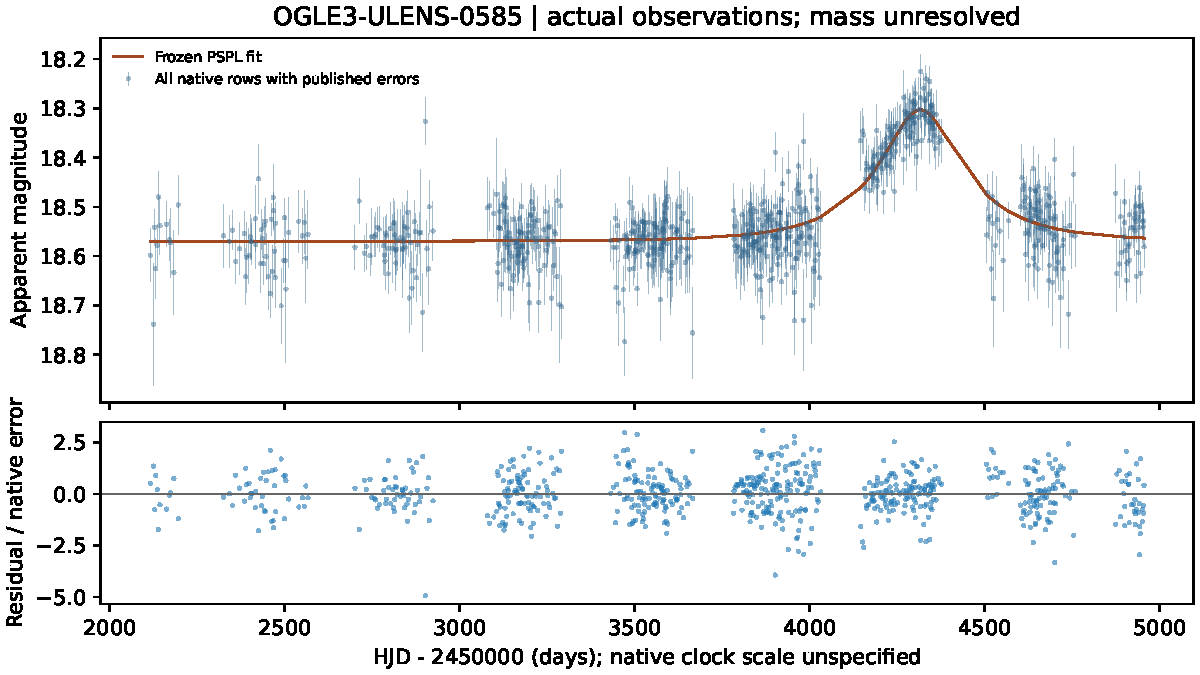
\includegraphics[width=.95\linewidth]{../figures/OGLE3-ULENS-0585_native.pdf}
\medskip
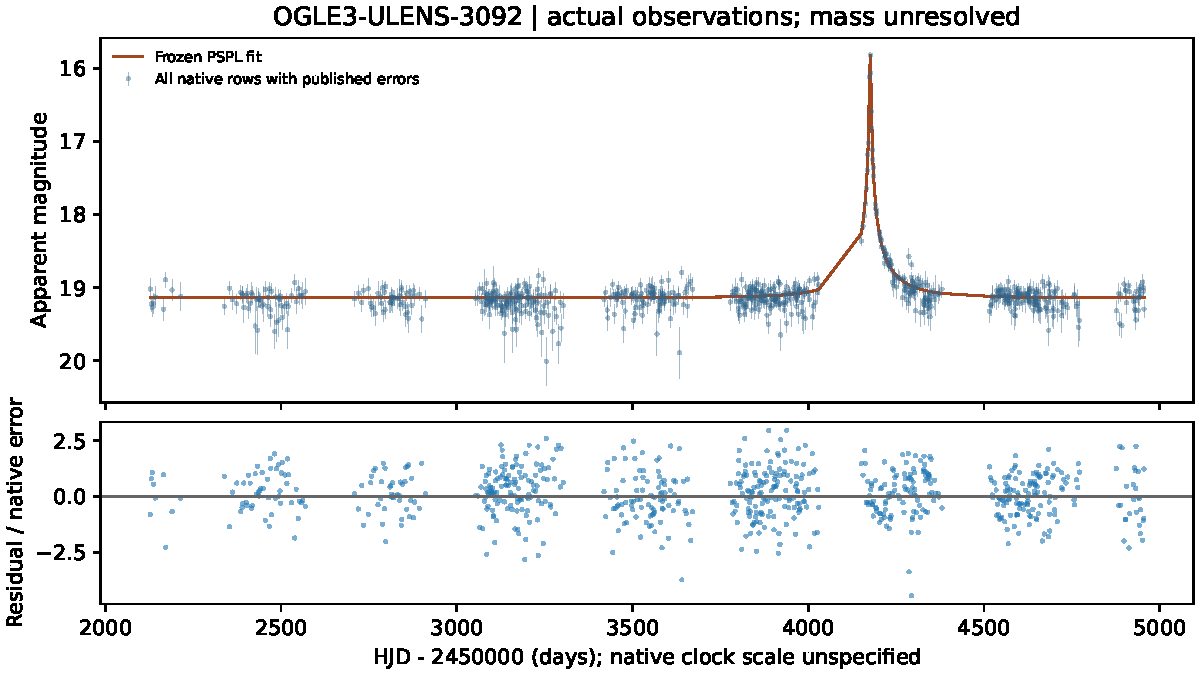
\includegraphics[width=.95\linewidth]{../figures/OGLE3-ULENS-3092_native.pdf}
\caption{Actual observations of the only two events passing the frozen
archival-follow-up screen. Curves are the saved baseline fits; bars are
the original magnitude errors, and lower panels retain all standardized
residuals. The fits identify conditional photometric combinations, not
lens mass or type. These historical events are not new discoveries.}
\label{fig:actual-followups}
\end{figure}

\begin{table}[tbp]
\centering\small
\caption{The only two events passing the frozen archival-follow-up
screen. Profile limits are nuisance-reoptimized $\Delta\chi^2=1$
reference crossings in days, without a coverage claim. Mass is
unavailable for both.}
\label{tab:pilot-followups}
\begin{tabular}{@{}lrrrr@{}}
\toprule
OGLE3-ULENS & Rows & $\chi^2/\nu$ & Fitted $t_E$ (d) & Profile (d)\\
\midrule
0585 & 734 & $748.247/729$ & 268.17 & $[202.91,344.96]$\\
3092 & 739 & $805.423/734$ & 187.73 & $[170.06,208.64]$\\
\bottomrule
\end{tabular}
\end{table}

The fitted baseline source fractions, 0.180 and 0.195, emphasize that
blending remains consequential. OGLE3-ULENS-0585 is catalog source
\texttt{BLG122.6.83113}; the supplied catalog has no EWS alias.
OGLE3-ULENS-3092 is \texttt{BLG225.6.198210}, independently associated
with OGLE-2007-BLG-057 by the official EWS coordinates (separation
0.75 arcsec). It is also MOA-2007-BLG-027, discussed by
Yock~\cite{Yock2008}; its prior high-magnification event and incomplete
peak coverage are not a new discovery. The historical EWS and optimized
catalog star identifiers belong to different reductions and are both
retained. Bounded alias/name/coordinate searches locate no specific
earlier lens-interpretation paper for 0585, but absence from this search
does not establish novelty. Neither object has measured mass here;
both are candidates for archival reanalysis and imaging feasibility,
not current alerts or credible new black-hole classifications.

The four exact prior-parallax matches in the full pilot are
0264/PAR-07, 0568/PAR-21, 2122/PAR-37 and 3404/PAR-17. In particular,
0264 was already proposed as a dark-remnant candidate in the 2016 study.
The later Gaia-informed analysis changes its conditional inference
\cite{Mroz2021}; a prior-dependent literature mass is not imported as
a mass measurement by this PSPL fit. Machine-readable literature
annotations preserve these associations alongside the unchanged frozen
results. The run yields zero mass-supported black-hole candidates and
zero new black-hole interpretations.

\subsection{The historical known-system benchmark and its stopping point}

OB110462 (OGLE-2011-BLG-0462/MOA-2011-BLG-191) is analyzed only with
the corresponding Zenodo 6607578 version 1.0.0 release
\cite{Lam2022Letter,Lam2022Supplement,Lam2022Data}, separately from the
pilot. The deposit's requested OGLE attribution is also retained
\cite{Udalski2015}. Its 15\,545 OGLE and 46\,040 MOA photometric rows
are retained. Later analyses use additional observations and revised
reductions \cite{LamLu2023,Sahu2025}; their masses and newer measurements
are not substituted for the 2022 input version.
All five specified PSPL fits converge with confirmed multistart solutions,
yet all fail the declared photometric adequacy screen and show
time-correlated/seasonal residuals (Table~\ref{tab:historical-benchmark}).
Convergence therefore cannot be presented as recovery of the published
black-hole mass. Parallax, source/lens complexity and noise calibration
require their own validated likelihoods.

\begin{table}[tbp]
\centering\small
\caption{Historical 2022-data benchmark: all entries are inadequate
photometry-only fits. The final column evaluates the native-error
$\chi^2$, including for the alternative weighting sensitivity.}
\label{tab:historical-benchmark}
\begin{tabular}{@{}lrr@{}}
\toprule
Fit/sensitivity & Fitted $t_E$ (d) & Native $\chi^2_\nu$\\
\midrule
Joint OGLE/MOA & 282.80 & 2.4515\\
OGLE only & 270.79 & 3.6754\\
MOA only & 299.06 & 2.0259\\
Equal-instrument objective & 276.47 & 2.4532\\
Signed-blend sensitivity & 282.80 & 2.4515\\
\bottomrule
\end{tabular}
\end{table}

Sixteen HST rows at eight shared visits are ingested with native column
labels, but are not used for precision joint inference. Primary-source
recovery establishes that the 2022 reduction applies a cross-filter
alignment, while a historical BAGLE reader converts private decimal-year
UTC epochs to MJD. Neither supplies the missing exact export mapping for
these deposited ASCII times. A concrete check against MAST observation
metadata finds all eight native numbers outside the matching F606W
exposure windows if naively interpreted as MJD UTC. No guessed epoch
shift or second filter offset is applied. Astrometric frame/coordinate
and covariance conventions also require verification before composition
with an ephemeris. The precision joint route consequently reports missing
verified metadata and leaves $\theta_E$, $\pi_E$ and mass unresolved.

Lam et al.'s published default weighting sums the photometric and
astrometric log likelihoods; their equal weighting divides each data-group
log likelihood by that group's count \cite{Lam2022Supplement}. The
photometry-only equal-instrument sensitivity above omits HST astrometry
and does not reproduce that published joint likelihood. This is a
version-specific benchmark of data admission and model failure, not a
replacement for either published mass analysis. The source/metadata
research, archived source hashes, raw-data provenance, all-event table,
fit diagnostics, residual plots and replay instructions are distributed
with the review material. Raw OGLE observations remain external pending
clear redistribution permission; the Zenodo deposit declares CC BY 4.0.

% Joint benchmark: compact public audit accompanies the frozen external outputs.
% Final source pins and completion receipts are bound by the release coordinator.
% Scientific source freeze: 5bb94198565fb25414f1f05908c00d49838c4b73.
% Authoritative prediction correction: JOINT_VALIDATION_PARTITION_V2_1_FREEZE.json.
\section{A separately versioned joint angular--photometric benchmark}
\label{sec:joint-native-benchmark}

The unresolved pilot does not identify a lens mass. We therefore evaluate a
separate angular--photometric route on the previously studied system
OGLE-2011-BLG-0462/MOA-2011-BLG-191 (OB110462). This is a known-system benchmark,
not an additional member of the frozen 100-event pilot and not a new discovery.
Its observations, calibrations, and analysis version are distinct from the
historical 2022 release discussed above. Published mass estimates are comparison
results; none is supplied as an observation, prior, initial mass, or acceptance
criterion. A successful analysis of this one positive system would establish
capability on this data version, rather than a population completeness,
false-positive rate, or general guarantee of black-hole identification.

\subsection{Native data, calibration, and time provenance}

The new version preserves all 15,533 author-reduced OGLE rows, with native HJD,
magnitude, reported uncertainty, seeing, and original line identity. The primary
published time window, HJD $2455376$--$2457700$, selects 12,500 OGLE observations;
the excluded rows remain available for the mandatory all-row sensitivity.
The 2023 author Table~2 supplies 21 HST filter observations at 11 calendar visits,
each with an east coordinate, north coordinate, magnitude, and respective
reported errors \cite{LamLu2023}. There are consequently 12,521 primary
photometric observations and 42 angular coordinate values. East denotes the
published tangent-plane $\alpha_* = \alpha\cos\delta$ coordinate; a second
$\cos\delta$ factor is not applied. These are unresolved observations, without
manufactured image positions, flux ratios, delays, distances, or covariances.

The author tables already include the stated neighbor-bias and additive error
calibrations. We do not repeat those corrections or reapply the older empirical
filter shift. Native errors remain immutable in the input, export, and replay.
The OGLE error calibration was designed to represent empirical observed scatter
by brightness and detector \cite{Mroz2022Noise}; it does not provide a unique
decomposition into independent and correlated noise. No full observational
covariance is supplied. Every fitted correlation or extra calibration term below
is therefore an explicit analysis hypothesis.

The HST table provides dates rather than precise combined-measurement epochs.
Program, date, filter, exposure count, and duration match 82 archived FLC primary
headers. We derive their UTC exposure midpoints, convert them to TDB, and average
the model over all corresponding midpoints for each angular datum. These
derived times are not represented as the authors' centroid weights. Duration
weights and the full exposure-window endpoints are mandatory sensitivities;
the largest visit window spans about 6061~s. The OGLE deposit does not specify
the underlying HJD clock scale. The primary import explicitly assumes HJD on
the UTC clock, inverts the heliocentric light-time correction, and converts to
observer JD on the TDB scale. A $\pm120$~s clock sensitivity is declared; no
resolution of the clock scale is implied. No unresolved 2022 ASCII time origin is repaired using the 2023
calendar dates.

The portable source pack contains the exact author table bytes, corrected OGLE
file, exposure-header prefixes, mapping, source URLs, licenses, and SHA-256
inventory. Its standard-library helper verifies the pack and can retrieve the
minimal header prefixes using checked HTTP range responses; full FLC images
are unnecessary. The two author data releases used here declare CC BY 4.0;
the HST header material has separate public-data provenance. Those terms do not
imply permission to redistribute every other OGLE product. The scientific source,
canonical numeric input hash, protocol, and transport files have independent
version pins. Native byte hashes survive browser transport unchanged.
We credit the OGLE team and Lam and Lu for the author reductions, and the
NASA/ESA Hubble Space Telescope and MAST for public WFC3 exposure metadata;
no new HST image reduction is claimed.

\subsection{Joint equations and identified quantities}

We use north--east vectors and define $\boldsymbol q$ from the lens to the
unlensed source, in units of the angular Einstein radius. With
$\boldsymbol n=(\cos a,\sin a)$, $\boldsymbol b=(-\sin a,\cos a)$, and the
heliocentric Earth position projected on the tangent plane in AU,
\begin{equation}
 \boldsymbol q(t)=u_0\boldsymbol b+
 \frac{t-t_0}{t_E}\boldsymbol n+\pi_E\boldsymbol p_\oplus(t),\qquad
 A(u)=\frac{u^2+2}{u\sqrt{u^2+4}},\quad u=|\boldsymbol q|.
 \label{eq:joint-native-trajectory}
\end{equation}
Here $t_0,u_0$ describe the rectilinear heliocentric trajectory, rather than the
apparent peak after annual parallax. The direction $a$ remains a fitted parameter
at $\pi_E=0$. For instrument $j$, baseline magnitude $m_{b,j}$ and source fraction
$g_j$ give
\begin{equation}
 m_j(t)=m_{b,j}-2.5\log_{10}\{1+g_j[A(u(t))-1]\}.
\end{equation}
For a dark lens and an unblended angular centroid, the image-summed displacement
from the unlensed source is \cite{DominikSahu2000}
\begin{equation}
 \boldsymbol\delta(t)=\theta_E\frac{\boldsymbol q(t)}{u(t)^2+2}.
\end{equation}
The measured centroid model adds a free source position, relative-frame proper
motion, relative-frame apparent parallax
$-\varpi_{S,\mathrm{rel}}[\boldsymbol p_\oplus(t)-\boldsymbol p_\oplus(t_{\rm ref})]$,
and the declared constant filter offsets. The linear angular nuisance parameters,
including $\theta_E$, are profiled within their physical analysis domain at each
nonlinear state. They are reprofiled when mass is fixed. Cross-filter angular
correlation and extra angular jitter are sensitivity assumptions, rather than
covariance claimed to be measured.

Independent annual-parallax and angular-scale information can then identify
\begin{equation}
 \pi_{\rm rel}=\theta_E\pi_E,\qquad
 M=\frac{\theta_E}{\kappa\pi_E},\qquad
 \kappa=\frac{4G}{c^2\,\mathrm{AU}}
       \simeq8.14385\,\mathrm{mas}\,M_\odot^{-1}.
 \label{eq:joint-native-mass}
\end{equation}
At zero or unidentified $\pi_E$, a finite mass is unavailable. Source and lens
absolute parallaxes, distance, and absolute proper motion remain unavailable
without an independently calibrated reference frame. Neither a long duration
nor an angular fit alone supplies the missing mass information.

Within BHSM, this is one compact-lens optical potential counted once. The ordinary
lensing fit is interpreted as the observable exterior lens response of the BHSM
object; it is not an additional core potential. These data do not identify a
horizon, membrane radius, nongeometric core state, or interior equation of state.

\subsection{Preserved failures and the prospective noise extension}

The first joint version is retained, including its failed adequacy checks.
Its native-diagonal fit had photometric $\chi^2=12573.2$ for approximately 12,510
degrees of freedom, but residual lag-one correlation $0.130$. A satisfactory
global quadratic alone therefore did not establish independent noise. Adding
an OU covariance to the full supplied diagonal reduced lag-one correlation to
$0.0181$, but yielded innovation $\chi^2=10720.2$ for approximately 12,508 degrees
of freedom. This severe lower-tail deficit was absent from 20 generated and
refitted controls (quadratic range $12255.9$--$12747.4$). The fitted covariance
family was inadequate; an upper-tail-only check would have concealed the failure.
The discrepancy is consistent with overcounting marginal scatter, but does not
uniquely establish its instrumental cause. The finite-difference coordinate
study also exposed a numerical time-step error. Earlier point estimates are
preserved as conditional diagnostic outputs, not accepted mass measurements.

These findings motivate version~2, internally frozen after version~1 exploration
and before its own measured fits at commit
\texttt{5bb9419}. This is a prospective post-diagnostic extension, not an external
preregistration. The complete candidate set comprises a centered-time diagonal
check (G0), a primary native-marginal OU hypothesis (G1), and an explicit fitted
calibration competitor (G2):
\begin{align}
 R_{ik}&=(1-f)\delta_{ik}+f\exp[-|t_i-t_k|/\tau],\\
 C_{\rm G1}&=S R S,\qquad S_{ii}=\sigma_i,\\
 C_{\rm G2}&=S_{\rm eff} R S_{\rm eff},\qquad
 (S_{\rm eff})_{ii}^2=k^2\sigma_i^2+s^2.
\end{align}
The fixed domains are $0\le f\le0.95$, $0.05\le\tau\le100$~d,
$0.5\le k\le2$, and $0\le s\le0.02$~mag. G1 preserves each reported marginal
variance exactly. G2 estimates a separate calibration hypothesis; it never
relabels its effective errors as supplied observations. These matrices replace
only the OGLE covariance block; HST photometry retains its reported diagonal
errors. Both minimize the full
Gaussian objective
\begin{equation}
 D=\boldsymbol r^{T}C^{-1}\boldsymbol r+
       \log\frac{\det C}{\det D_{\rm native}}+
       \chi^2_{\rm angular},
\end{equation}
with the exact, potentially negative relative log determinant. A bounded constant
offset permits a real least-squares representation and is subtracted from every
reported deviance. The OU calculation is checked against dense covariance
algebra, including duplicate epochs and the $f=0$ and calibration-null cases.
Changing the numerical time center preserves the physical model; future targets
must supply their own physical time bounds and initial guesses.

\subsection{Prediction, controls, profiles, and stopping}

The fixed diagnostics screen both quadratic tails, lag correlations, and
Ljung--Box structure. Native-error, seeing, noise-free model-brightness quartiles,
fixed event/off-event windows, and Julian seasons test residual structure with
declared multiplicity qualification. Observed-magnitude bins do not gate a naive
quadratic check, because they select residual tails. These postfit screens are
approximate; generated and refitted controls assess their behavior.

Independent driver review found that the originally specified
$\lfloor\mathrm{JD}_{\rm TDB}-0.5\rfloor$ day boundary split Chilean observing
nights: 154 adjacent train/validation pairs were separated by less than 0.1~d.
That original conditional score is retained with its limitation. Before any
prediction outcomes, a separately recorded version~2.1 correction fixed the
observing-night unit at local mean solar noon,
$N=\lfloor\mathrm{JD}_{\rm TDB}+\lambda/360^\circ\rfloor$, with the Las Campanas
longitude and $N\bmod5=0$ held out. The corrected set contains 2464 OGLE rows;
all HST rows remain in training. Its minimum adjacent cross-partition gap is
$0.6063$~d, with no pairs below 0.25~d. The official observatory longitude and the
driver's approximate site longitude produce identical row identities.

At the same training-only fitted physical and covariance state, the exact
conditional photometric quadratic is $Q_{\rm all}-Q_{\rm train}$ and the relative
determinant is
$\log\det C_{\rm all}-\log\det C_{\rm train}-\log\det D_{\rm held}$.
This retains GP correlations across the partition. Angular objective terms are
excluded from the difference. Independent dense Schur-complement tests agree to
$1.2\times10^{-14}$. Plug-in prediction probabilities do not account exactly for
estimated mean and covariance uncertainty and are not Bayesian evidence.

The protocol fixes at least 20 full-cadence generated/refitted controls per OU
candidate, their seeds, multistart modes, mass profiles, and mandatory timing,
frame, calibration, blend-location, ephemeris, and all-row sensitivities. Twenty
controls resolve Monte Carlo tails only to $1/21$ and do not certify interval
coverage. Mass support requires resolved competing minima and finite profile
crossings, adequate residual and prediction checks, and stability across the
declared sensitivities. Numerical caps and unresolved searches interrupt support;
physical nuisance boundaries preclude automatic Wilks coverage. If every fixed
candidate fails, this campaign stops with a conditional or inadequate mass result.
Further outcome-driven model revision is not an acceptance requirement.

\subsection{Verified campaign outcomes and scope}

All 16 starts per candidate converged after the declared continuation, but all
three candidates failed baseline adequacy. Table~\ref{tab:joint-failed-candidates}
retains their conditional point estimates; these are not accepted measurements
and their spread is not an uncertainty interval.
\begin{table}[htbp]
\centering
\caption{Frozen joint candidates after declared continuation. Each angular
quadratic is approximately $32$ for 29 conservatively counted degrees of freedom.
All candidates fail the residual-structure gate.}
\label{tab:joint-failed-candidates}
\begin{tabular}{lrrrr}
\hline
Candidate & Conditional $M/M_\odot$ & Photometric $Q/\nu$ & Lag one & Failed bins\\
\hline
G0 & 6.546 & $12568.56/12510$ & 0.1295 & 15\\
G1 & 7.103 & $12598.17/12508$ & 0.0198 & 15\\
G2 & 18.061 & $12528.74/12506$ & 0.0464 & 8\\
\hline
\end{tabular}
\end{table}

\begin{figure}[htbp]
\centering
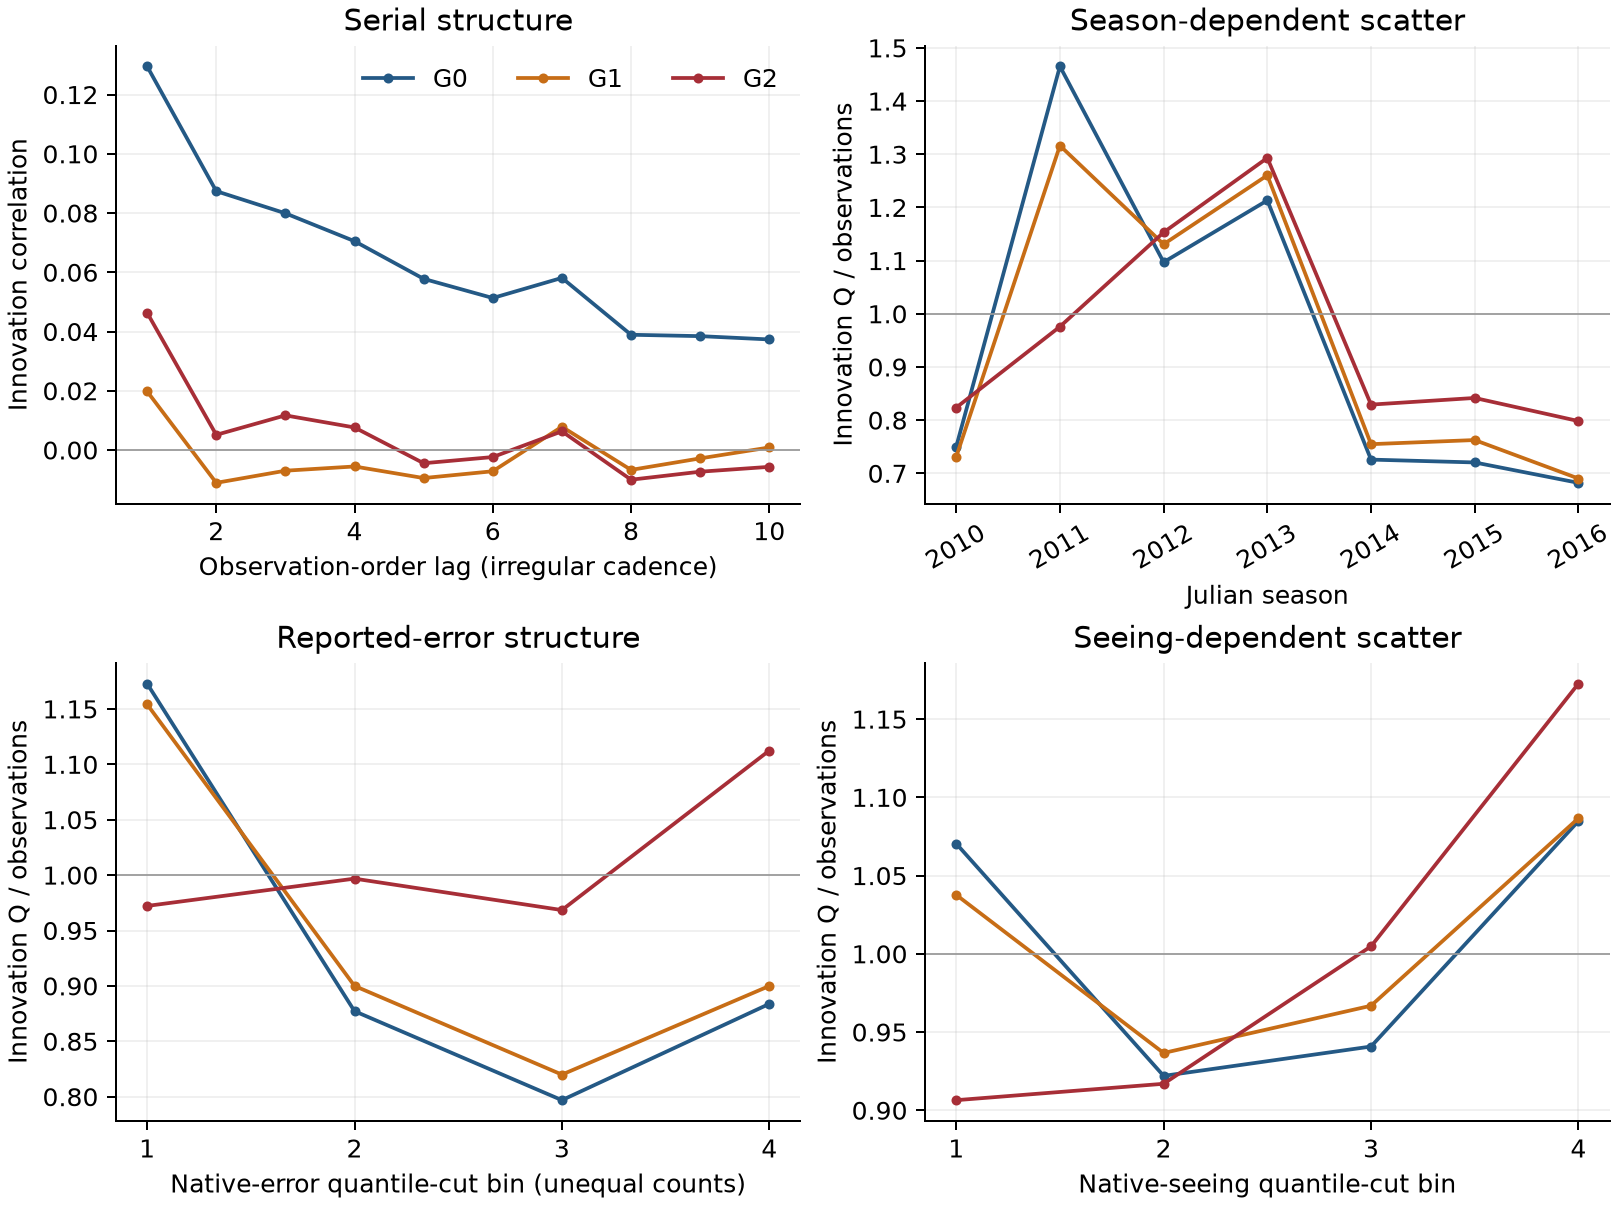
\includegraphics[width=\linewidth]{../joint_known_system_20261022/joint_noise_diagnostics.png}
\caption{Residual structure for the three frozen joint candidates, after the
declared continuation. Global quadratics conceal season, reported-error and
seeing dependence. The reported-error quantile cuts have tied rounded values
and unequal counts $(5817,2874,1787,2022)$; they are not equal-sized samples.
These diagnostic ratios are not calibrated confidence bands.}
\label{fig:joint-noise-failure}
\end{figure}

G0 retains strong serial dependence. G1 removes most short-lag structure and
passes the approximate Ljung--Box screen, but fails native-error, model-brightness,
seasonal, and event/off-event residual checks. G2 fails brightness, seeing, and
seasonal checks, has Ljung--Box probability $6.77\times10^{-5}$, and reaches the
artificial 100~d OU timescale cap. Its lower objective does not establish an
adequate likelihood or a physical timescale limit. Every global quadratic is
apparently acceptable; the failed structure demonstrates why those scalar values
cannot establish trustworthy physical uncertainty.

The corrected whole-night conditional quadratics are $2647.64$ (G1) and
$2540.41$ (G2) for 2464 held-out rows, with approximate two-sided probabilities
$0.01038$ and $0.2771$. Both clear the declared $0.01$ plug-in screen, G1 narrowly.
Their relative Gaussian predictive deviances are $2523.02$ and $2245.68$.
Prediction success cannot override the failed full-data and training residual
structures or the G2 numerical cap. Independent reevaluation of the three saved
baseline states and two saved prediction scores reproduces every checked
quadratic, determinant, and score exactly without refitting.
The original midnight-boundary diagnostics are also retained: for 2467 held-out
rows, G1 has $Q=2710.21$ and approximate probability $0.000768$, while G2 has
$Q=2596.51$ and probability $0.06846$. These values do not supply a whole-night
validation, because that partition splits actual observing nights.

Both fixed 20-control sets are complete. None of the 40 generated/refitted cases
fails a declared residual-variance bin; 19 of 20 in each family pass the overall
screen, with the remaining case rejected by its angular quadratic. Each generated
control family's pass fraction $19/20$ has an exact 95\% binomial interval $[0.751,0.999]$ for
its local generating-model pass probability, rather than mass-interval coverage.
Each measured
lag-one correlation exceeds all 20 corresponding generated values. G1's measured
held-out quadratic also exceeds all its generated values, despite narrowly
passing the plug-in screen. These comparisons reinforce the limitations of a
single scalar screen, but provide only the coarse $1/21$ Monte Carlo tail
resolution. They are local generating-mode checks, rather than global search
or confidence-coverage certification. Ten G2 generating-mass profiles encounter
the numerical timescale cap and remain interval-ineligible.

The completed serial mass grids retain 31 points per OU candidate, without
cross-mass warm starts. G1 has 24 locally eligible and seven cap-limited rows;
crossing refinement gives conditional support $5.989$--$8.399\,M_\odot$ at
$\Delta D=1$ and $5.021$--$9.910\,M_\odot$ at $\Delta D=3.841459$.
These are diagnostic likelihood supports under an inadequate noise hypothesis,
not accepted confidence intervals. Every G2 grid row is cap-limited, and its
32-point refinement gives no eligible crossings or conditional support interval.
An auxiliary parallel scheduling check preserves
the serial results as authoritative: all compared admission states agree, but
some optimizer values differ by up to $0.0133$ in deviance across thread
environments. Three separately repeated points with the same one-thread setting
are identical. No cross-platform numerical identity or profile coverage is
inferred from those checks.

The conditional angular scales range from $4.77$ to $5.18$~mas, whereas the
conditional parallaxes range from $0.0324$ to $0.0971$ and the timescales from
$282.4$ to $340.5$~d. The narrower variation in angular scale is a description of
these fitted models, rather than a validated systematic error bound. In
particular, their mass ratio is not stable across the fixed noise hypotheses.
The software recovers conditional trajectories and angular signals, but this
campaign does not identify a reliably calibrated mass or mass interval.

The protocol therefore stops mass acceptance for every fixed candidate. Diagnostic
profiles and generated controls remain auditable; no additional covariance family
is introduced to make an expected mass appear. Sensitivity calculations cannot
convert an already inadequate baseline into accepted physical inference.
The additional version~2 timing/frame/blend sensitivities are not executed,
because baseline adequacy is their declared entry gate; no robustness to those
systematics is claimed. Earlier version~1 diagnostic sensitivities remain
separately preserved. The
known-system analysis consequently provides no positive demonstration that this
engine can reliably classify unknown black holes. It does demonstrate native-data
ingestion, physical forward prediction, explicit failure detection, and replay.

For a previously unknown object, mass support above a declared compact-object
threshold would still require independent darkness/lens-flux and single-lens
compatibility evidence before a black-hole interpretation. Published darkness
arguments for OB110462 \cite{LamLu2023} are separately attributed; this engine
does not manufacture a new lens-flux limit or assume an absolute distance.
The benchmark does not retrospectively turn the pilot's two archival follow-up
light curves into mass measurements or new black-hole discoveries.

Useful next calibration evidence includes documented
OGLE clock and per-exposure variance components, matched-star and seeing/detector
diagnostics, and exposure-level HST astrometric covariances, reference transforms,
bias corrections, and epoch weights. Absolute frame calibration is separately
required before distance or absolute motion. A new unknown-system interpretation
also needs measured angular-parallax information and independent lens/source
flux constraints. A present-day image cannot manufacture the missing angular
trajectory around a historical photometric peak. These are observational and
calibration requirements, rather than permission to iterate the model until a
black-hole claim passes.

Rejecting these covariance hypotheses does not prove that every estimator using
the observations must fail. Correct-mean estimating equations with cluster/block
robust inference are a separate possible route \cite{LiangZeger1986,CameronMiller2015}.
They still need justified mean/exogeneity and between-block dependence assumptions,
and finite-sample validation for the sparse, unevenly informative HST visits.
Robust uncertainty does not correct a biased mean or shared frame calibration.
No such alternative mass estimator is fitted or validated here, and no reliable
mass support is inferred from the saved G0 point alone.


\section{Candidate localization without a precise mass}
\label{sec:candidate-inventory}

Candidate selection and localization are useful results before an individual
mass is identified. They require distinct evidence labels: a \emph{supported
lensing event} has evidence for lensing; a \emph{black-hole search target}
justifies further investigation; a \emph{black-hole candidate} requires
specific evidence favoring that interpretation, with alternatives retained;
and a \emph{strongly supported identification} requires discriminating
evidence against relevant stellar and other compact-object explanations.
A precise mass is not required for a search target. Lensing itself is not
a black-hole classification, and nonrejection of one light-curve model is
not a comparison against source variability or other alternatives.
\emph{Review required} therefore remains an available outcome.

\subsection{A complete, versioned historical inventory}

The metadata inventory joins the complete 100-event pilot to all 59
published parallax events of Wyrzykowski et al.\ \cite{Wyrzykowski2015,Wyrzykowski2016}.
Four shared identities---0264/PAR-07, 0568/PAR-21, 2122/PAR-37 and
3404/PAR-17---are independently checked using database identifiers,
published aliases and compatible catalog directions. The union contains
155 events. It retains all 89 inadequate pilot fits, all 11 scalar-screen
nonrejections and both stricter frozen follow-up qualifications.
The parallax cohort retains all 142 published degenerate model summaries;
they are literature metadata, not additional observations.
Its 13 historical dark-remnant-consistent events are not 13 black holes:
that category includes white dwarfs and neutron stars and depends on the
adopted Galactic and relative-motion assumptions \cite{Wyrzykowski2016}.

Twenty-six exact database matches have independently hash-verified older
2015 photometry: 23 optimized Class A tables and three Class B tables,
containing 19\,068 rows. The remaining 33 entries stay explicitly
unavailable. These older tables are not asserted equivalent to the
2016 reduction, calibration or outlier masks. No new parallax fit,
population inference or follow-up ranking is performed by this inventory.
The earlier pilot ranking remains separately versioned.

\begin{table}[tbp]
\centering\small
\caption{Three investigation targets with distinct evidential bases.
Coordinates are printed catalog source/event directions, with J2000
equinox; an observing epoch or current lens position is not supplied.
No row is an accepted new black-hole identification.}
\label{tab:atlas-targets}
\begin{tabular}{@{}lllp{.40\linewidth}@{}}
\toprule
OGLE3-ULENS & RA (h:m:s) & Dec (d:m:s) & Basis and limitation\\
\midrule
0585 & 17:48:45.32 & $-$34:44:43.8 &
Frozen photometric follow-up screens; mass and lens type unresolved.\\
3092 & 18:04:17.03 & $-$27:36:35.8 &
Same screens; known OGLE-2007-BLG-057/MOA-2007-BLG-027 event.\\
PAR-13 & 17:35:55.95 & $-$27:16:02.1 &
Disputed prior-conditional BH-scale interpretation; unreliable source
astrometry and a lower-mass alternative.\\
\bottomrule
\end{tabular}
\end{table}

\subsection{Literature revisions and localization limits}

The two pilot targets in Table~\ref{tab:atlas-targets} are qualified
archival follow-ups, not evidence that black holes are preferred.
PAR-13 enters as a disputed literature search target. The later analysis
of Mr\'oz and Wyrzykowski \cite{Mroz2021} revises several earlier
mass interpretations: PAR-02, historically the strongest black-hole
candidate, is favored to be a roughly $0.9\,M_\odot$ bulge star under
their fiducial priors. Their BH-scale PAR-13 inference depends on a
Gaia DR2 source solution with RUWE 1.67, absent from EDR3; an alternative
OGLE source proper motion gives a lower conditional mass. These
conflicting, prior-dependent interpretations remain attributed literature
records. They are neither independent lens-mass measurements nor optimizer
targets. None of the 155 entries is promoted to the candidate or strongly
identified black-hole tier by the tracker.

\begin{figure}[tbp]
\centering
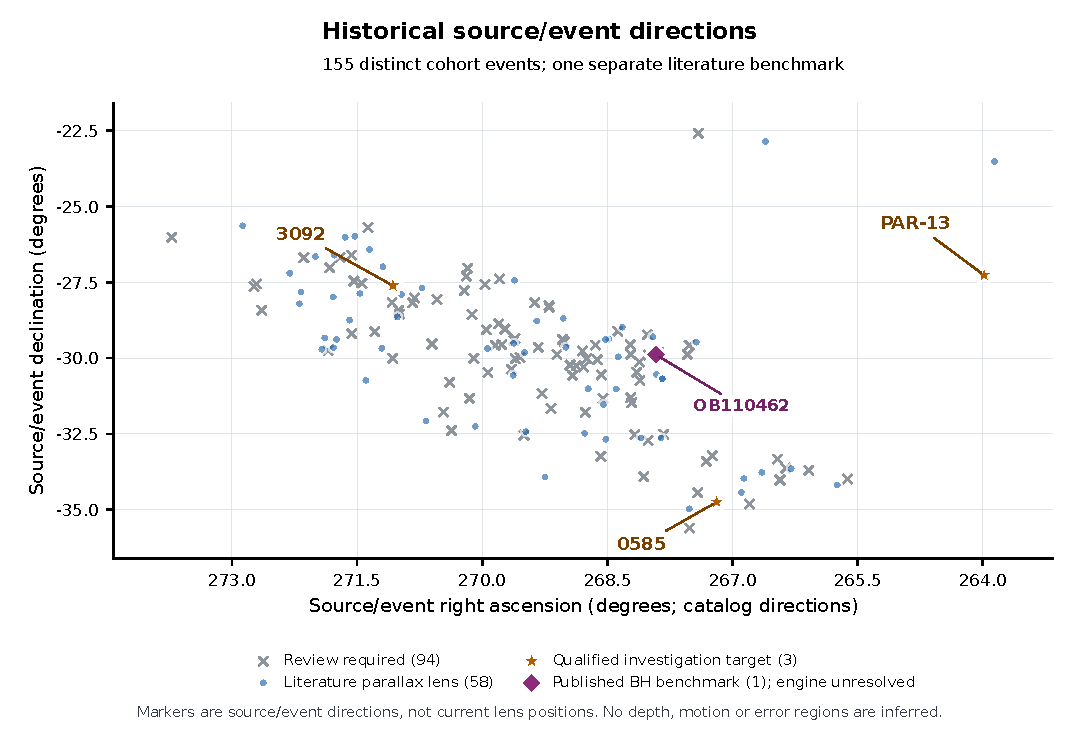
\includegraphics[width=.97\linewidth]{../figures/candidate_inventory_sky.pdf}
\caption{Historical source/event directions in the 155-event union,
with the separate published OB110462 benchmark optionally included
(156 markers in total). Supported-lens labels are inherited from the
published parallax study; review labels preserve the pilot's unresolved
assessments. The three search targets have different qualifications
(Table~\ref{tab:atlas-targets}). Markers are not present-day lens positions;
angular uncertainty regions, depth and propagation are unavailable.
Survey selection and alignment affect this footprint: an unmarked region
does not imply absence of black holes.}
\label{fig:candidate-inventory-sky}
\end{figure}

Source/event direction, inferred lens position at a stated epoch, and
three-dimensional position are separate outputs. A J2000 catalog label
specifies an equinox, not an observation epoch or proper-motion
correction. Every newly inferred lens position, uncertainty, mass,
distance, absolute proper motion and radial velocity remains null here;
no three-dimensional or propagated lens marker is supplied.
OGLE-2011-BLG-0462/MOA-2011-BLG-191 is a separate published positive
benchmark \cite{Sahu2025}. Its strong identification is labeled
\emph{literature}; the tracker's joint recovery remains unestablished.
The published full analysis is not certified by importing that label.
BHSM interpretation remains one ordinary compact-lens Einstein/GHY
exterior response counted once; these directions and screening results
identify no core state, membrane deformation or horizon.

\subsection{Usable and auditable metadata replay}

The app, \texttt{blackhole-tracker atlas} commands and Python interface
expose the same retained inventory, aliases, quality flags and evidence
layers. Filters select a view without deleting unselected or failed
records. A portable standard-library builder reruns association and
classification rules from factual metadata snapshots, with no original
observation redistribution or new likelihood call. Two assemblies are
byte-identical; relocation tests forbid reads of the original source
paths. Browser--Python replay preserves the exact UTF-8 inventory text,
including line endings, and checks selected records against the complete
inventory. SHA-256 establishes byte consistency, not authenticity,
scientific adequacy or black-hole certification. The software,
metadata and reviewer materials cite the
\href{https://github.com/ncarberry64/Berger-Hopf-Standard-Model}{formal BHSM repository}.


\section{What could actually be tracked?}

The resolved-pair product demonstrates compact-lens inference under its
declared synthetic measurement and covariance model. The separate
observational pilot demonstrates native-data ingestion, audited
photometric screening and honest unavailable mass outputs. It identifies
two historical archival-follow-up targets, but no mass-supported new
black-hole interpretation or detectable BHSM envelope. The separate known-system
joint benchmark also fails its declared noise-adequacy gates. Its conditional
mass points do not establish a reliable known-black-hole measurement or
reliability for unknown systems. The earlier broad information
scan has a distinct limitation. For the illustrative cosmological mass and transverse
speed $300$ km s$^{-1}$, ten observer years move the center only
$0.00236$ pc, or $6.95\times10^{-6}r_E$. Traversing the broad synthetic
$3.6r_E$ scan at that speed would take about $5.2$ million observer years.
The short-span design has nearly dependent columns; its released
spectrum must not be promoted into a realistic parameter forecast.
Several independent source configurations could sample a broad spatial
range, but that would require an actual source population, their
redshifts and a corresponding data model. It is not automatically
supplied by nine synthetic points.

A translated static profile is an adiabatic template evaluated at lens
crossing time. It requires slow motion, control of coefficient evolution
over the relevant crossing times, and control of scalar propagation.
For the speed example $v/c\simeq10^{-3}$, even nominal relative
corrections at that level cannot be ignored when claiming the tiny
subleading delay. Positive leading principal coefficients establish the
local branch's hyperbolicity/ellipticity conditions; they do not prove
global nonlinear stability, a UV completion or horizon admissibility.
Fast intrinsic deformation or ringdown needs a causal metric solution.
Such time-dependent black-hole lensing already has separate explicit
models \cite{Pantig2026}; they do not close the R1 matching problem.

The unknown flux is especially consequential. The regular-body integrated
source equation supplies one proxy, whereas a black-hole exterior has
an integration constant that must be selected by horizon, interior and
cosmological boundary conditions. The searched BHSM record did not
establish that selection. A surface-acceleration identity or a
Brown--York energy inversion on a known Schwarzschild worldtube does
not determine this scalar flux or its deformation response. Nor can the
two odd line-of-sight tensor modes be reconstructed by improving the
precision of the same static projection.

This missing evaluation is specific to the present action and background.
Cosmologically induced black-hole charges have been derived in related
shift-symmetric Horndeski models \cite{Babichev2025}, and regular stable
quasi-stationary cubic-Galileon black holes with cosmological asymptotes
have been constructed \cite{Smulders2026}. Those works provide a concrete
matching strategy. The explicit self-accelerating cubic de Sitter
constructions are not the present canonical-sign, linear-potential, rolling
matter background; directly substituting the latter coefficients into
that self-accelerating branch does not give a real Hubble parameter.
Their results therefore cannot simply select the flux proxy used here,
nor do they provide this paper's normalized quadrupole state.

Even perfect matching and a detectable transfer would track an exterior
compact-mass/envelope combination. Any alternative interior producing
the same Weyl response on every sampled ray gives the same data. A
horizon claim therefore needs additional physics or independent
observables. Unrestricted source transformations, line-of-sight
potentials, uncertain distances, evolving macrostructure and flux
propagation effects can also change the finite-family inference result.
Multiple source redshifts alone do not remove every such freedom.

\section{Discussion and conclusions: scientific advance and limits}

Static cubic screening, its multipole powers and exact Green functions
are established \cite{Kimura2012,Chu2013,Brito2014,Kobayashi2026}.
General STF gravitational multipole projection is also established
\cite{Turyshev2022}. The point-mass delay/flux estimator is standard,
and ordinary radial multipole separation and profiled linear inference
are standard methods. We do not claim priority for those ingredients.

The addition combines their normalized R1 optical composition with an
exterior-wide sufficient state cap and a runnable compact-lens inference
workflow. Its theory exposes a delay-blind leading response, an exact
apparent-mass/shear degeneracy and line-of-sight nulls. Its product retains
full covariance and source freedom for resolved pairs, and reports
historically versioned synthetic recovery with limited local-interval
coverage checks. Its new unresolved route preserves native observations
and carries every pilot outcome, including inadequate models and
unavailable physical quantities, into the released table. The finite harmonic control makes a cause ambiguity exact
rather than assigning every structured residual to BHSM.

The result supports a theoretical and computational lens-modeling methods
paper with a usable BHSM-interpreted research tool and a bounded
observational screening pilot. Ordinary mass/motion recovery remains
useful when identified by suitable data; unresolved light-curve
timescales alone do not supply it. Under the author's surface definition,
supported gravitational geometry is already interpreted as BHSM surface
topography. Such configuration inference can guide investigation before
its unique physical identity is established; the conditional pilot fits
alone do not validate a gravitational origin. Agreement with the Einstein-sector
response is allowed; it does not uniquely select the underlying theory. The present results do not establish
an independently detected R1 deformation, horizon classification or a decisive new
astrophysical discovery. Further R1 prediction needs a normalized
black-hole/homogeneous-background boundary map selecting exterior flux
and deformation dynamics. Resolved-pair use requires calibrated
positions, geometric fluxes, delays and an adequate environmental model.
Unresolved mass inference requires independent angular-scale and
parallax information, verified clocks/frames and a validated joint
likelihood. The two frozen pilot follow-ups warrant archival and imaging
feasibility checks; their ranking supplies no mass or BHSM-specific
detection. The expanded 155-event atlas adds PAR-13 as a differently
qualified, disputed literature search target. Its three investigation
targets are not three independently identified black holes. All
unassessed and failed cohort cases remain visible, and the published
known-system benchmark stays outside the cohort ranking. No new
telescope detection or journal submission is reported.

The current-kernel study completes its full frozen accounting but rejects three
photometric uncertainty-calibration tests. Successful conditional resolved
controls therefore do not establish universally calibrated errors or a
black-hole classifier. The separately normalized Student experiment likewise
does not clear its numerical-resolution gate; an eligible conditional point
near a published mass is insufficient to count as independent recovery.
Neither result clears the scientific publication hold.

The completed Gaussian joint candidate set stops without an accepted mass. Its apparently
satisfactory global quadratics and whole-night predictive screens cannot override
failed residual structure or a numerical covariance-timescale cap. Valuable
further evidence includes per-exposure variance, seeing/detector diagnostics,
astrometric covariance and reference-frame information. A separate robust
estimating-equation route would need its own justified mean/dependence assumptions
and finite-sample validation; this campaign does not evaluate it. A known system's published classification
is separately attributed and does not certify this engine; one successful system
would also be insufficient to establish population reliability.

\paragraph{Data and code availability.}
The formal reviewer repository is
\href{https://github.com/ncarberry64/Berger-Hopf-Standard-Model}{Berger--Hopf Standard Model},
with the product under \nolinkurl{products/blackhole_tracker/} and this
paper under \nolinkurl{papers/bhsm_blackhole_tracker_20261021/}.
The integration branch is
\href{https://github.com/ncarberry64/Berger-Hopf-Standard-Model/tree/codex/blackhole-tracker-real-data-20261022}{the real-data integration branch};
the separate Manuscript-Generation repository is a development workspace.
The rc7 resolved, native-photometry, joint, candidate-inventory and
measured angular-track product source is pinned to formal revision
\href{https://github.com/ncarberry64/Berger-Hopf-Standard-Model/tree/f90c9dc4a9eed262ca3b2291b3320f47bb4a5333/products/blackhole_tracker}{\texttt{f90c9dc4a9ee}}.
Its product \texttt{CITATION.cff} records version 0.2.0rc7 separately from
the historical repository DOI. Both original legal notices accompany the
wheel and source distribution; their terms are unchanged. The preceding
RC6 source revision \texttt{4c71556f5ab4} remains preserved.
The final release receipt pins the completed source revision, wheel,
manuscript PDF and CI outcomes. The theory/source reconciliation is
independently pinned to formal revision
\href{https://github.com/ncarberry64/Berger-Hopf-Standard-Model/tree/705d4c7e2f9a832b457f63ff975e7d4dc8008645}{\texttt{705d4c7e2f9a}}.
Earlier synthetic/theoretical projects and their receipts remain
versioned historical material.

The original OGLE project supplies the native pilot observations
\cite{Wyrzykowski2015}; the 2022 benchmark is Zenodo 6607578 version
1.0.0, declared CC BY 4.0 \cite{Lam2022Data}. For this pilot and older
benchmark, native source files remain
external and unmodified; the distribution provides source URLs, required
citations, hashes and fetch/replay instructions. Raw OGLE redistribution
is not assumed from download access. The public
\texttt{real\_data\_pilot\_20261022/} directory contains the frozen protocol,
source/kernel pins, compact all-event results, profiles and fit
diagnostics, all 100 residual plots, historical benchmark results and
separate literature annotations. Complete native rows and source-line
identities are retained in external replay products. Source recovery and
metadata gaps are documented with archived primary-source hashes.
Theoretical replay uses \texttt{scripts/reproduce.py}; product validation
and interface instructions are in the product README. The installed
app's analysis export is replayable through
\texttt{python -m bhtracker replay analysis.zip -{}-output replayed};
the native route preserves its data contract, original source identity,
BHSM interpretation and unavailable mass fields.

The separate \texttt{candidate\_atlas\_20261023/} metadata package supplies
the exact inventory, offline builder, factual source snapshots, source
hashes and independent portable-rebuild checks. It preserves the 100-event
pilot outcomes and all 59 published parallax records with four verified
shared identities. The atlas runs through the local browser, CLI, Python
API and fifth notebook. Its JSON replay retains all 155 cohort records,
the separate benchmark and exact original UTF-8 inventory bytes even
when the view selects only three targets. Catalog source/event directions
are not measured present-day lens positions. Raw photometry and published
conditional masses are not manufactured to populate unavailable fields.

The separate \texttt{joint\_known\_system\_20261022/} audit provides the
2023-data joint equations, fixed candidate protocol, partition correction,
compact results and residual diagnostics, source-pack manifest and rights,
independent computational reviews, and portable reproduction instructions.
The source pack preserves the CC BY 4.0 author observations
\cite{Mroz2022Data,LamLu2023} and separately attributed public HST header
metadata. Its source version does not replace the frozen 2022 benchmark or
100-event pilot. Final release metadata pins the formal BHSM code revision;
the development-workspace scientific freeze is separately recorded in the audit.

\paragraph{Author contributions.}
Conceptualization, methodology, formal analysis and writing:
Norman P. Carberry. Software, validation and visualization were prepared
with the AI/tool assistance described below. Scientific responsibility
and final manuscript approval rest with the author.

\paragraph{Funding.}
This research received no external funding.

\paragraph{Conflicts of interest.}
The author declares no conflicts of interest.

\paragraph{Institutional review board and informed consent.}
Not applicable. This theoretical and computational study uses synthetic
validation measurements and public archival astronomical observations;
it introduces no human-participant or animal research.

\paragraph{Acknowledgments and AI/tool disclosure.}
During preparation of this manuscript and study, OpenAI ChatGPT and
Codex (GPT-6 model family) were used for source recovery, symbolic
calculation and checking, software generation and revision, numerical
verification, visualization, literature checking and manuscript drafting.
Retained claims are supported by the stated mathematics, source records
and executable checks; AI output is not independent physical evidence.
Independent agent reviews are internal computational checks, not external
peer review. Responsibility for the retained scientific content rests
with Norman P. Carberry.

\appendix
\section{First variation of the delay--flux mass estimator}
\label{app:estimator-variation}

The point-mass delay relation is standard; see, for example,
Mu\~noz et al.~\cite{Munoz2016}. This appendix derives its first variation
under a general local lens-potential perturbation, including the displacement
of the images in the magnification calculation. The result is a thin-lens
projection rule; it selects neither a horizon response nor a physical
surface-state amplitude.

Use the reference point-mass Einstein angle and observed time scale
\begin{align}
 \theta_E^2=\frac{4GM}{c^2}\frac{D_{ls}}{D_lD_s},
 \qquad t_M=\frac{4GM}{c^3}(1+z_l),\notag\\
 \qquad \boldsymbol x=\boldsymbol\theta/\theta_E,
 \quad \boldsymbol y=\boldsymbol\beta/\theta_E.
 \label{eq:estimator-scales}
\end{align}
Hold the physical source, body mass, distances, redshift and screen fixed
while varying the dimensionless potential,
\begin{equation}
 \tau_\epsilon(\boldsymbol x;\boldsymbol y)
 =\tfrac12|\boldsymbol x-\boldsymbol y|^2-\ln r
  -\epsilon p(\boldsymbol x),\qquad r=|\boldsymbol x|.
 \label{eq:estimator-fermat}
\end{equation}
For $u=|\boldsymbol y|>0$, put $s=\sqrt{u^2+4}$. On the source axis the
reference images are $x_+=(u+s)/2>1$ and $x_-=-1/x_+<0$. Continue the
positive-parity minimum and negative-parity saddle without crossing a
critical curve or reversing their flux/time ordering. With
$R=|\mu_+|/|\mu_-|>1$ and $\Delta t=t_M(\tau_--\tau_+)>0$,
\begin{align}
 \ln R_0=4\operatorname{asinh}(u/2),\qquad
 h(u)=\tfrac12us+2\operatorname{asinh}(u/2),\notag\\
 M_{\rm app}=\frac{c^3\Delta t}
 {4G(1+z_l)h[2\sinh(\tfrac14\ln R)]}.
 \label{eq:estimator-standard}
\end{align}
Indeed, the lens equation $x-u-1/x=0$ gives
$\mu_+=x_+^4/(x_+^4-1)$, $\mu_-=-1/(x_+^4-1)$ and
$\tau_--\tau_+=\tfrac12(x_+^2-x_+^{-2})+2\ln x_+=h(u)$.
The distance factors in the physical time prefactor cancel against
$\theta_E^2$, so $M_{\rm app}=M$ for every reference alignment. The
aligned Einstein-ring limit is excluded from the two-image estimator.

Let $\delta=\partial_\epsilon|_0$ and define
\begin{equation}
 H_0(\boldsymbol x)=D^2\ln r
 =\frac{I}{r^2}-\frac{2\boldsymbol x\boldsymbol x^T}{r^4},
 \qquad A_i=I-H_0(\boldsymbol x_i).
\end{equation}
Differentiating the stationary lens equation at fixed $\boldsymbol y$ yields
\begin{align}
 \delta\boldsymbol x_i=A_i^{-1}\nabla p(\boldsymbol x_i),\qquad
 \delta A_i=-D^2p(\boldsymbol x_i)
             -DH_0(\boldsymbol x_i)[\delta\boldsymbol x_i],\notag\\
 \delta\ln|\mu_i|=-\operatorname{tr}(A_i^{-1}\delta A_i).
 \label{eq:estimator-total-hessian}
\end{align}
The evaluation-point term is essential. Explicitly,
\begin{align}
 DH_0(\boldsymbol x)[\boldsymbol v]&
 =-\frac{2(\boldsymbol x\cdot\boldsymbol v)I}{r^4}
 -\frac{2(\boldsymbol v\boldsymbol x^T+\boldsymbol x\boldsymbol v^T)}{r^4}\notag\\
 &\quad+\frac{8(\boldsymbol x\cdot\boldsymbol v)
                 \boldsymbol x\boldsymbol x^T}{r^6}.
\end{align}
Stationarity removes image displacements from the first arrival-time
variation, giving $\delta(\tau_--\tau_+)=p(\boldsymbol x_+)-p(\boldsymbol x_-)$.
Since $h'=s$ and $(\ln R_0)'=4/s$, the total estimator variation is
\begin{equation}
 \boxed{\displaystyle
 \delta\ln M_{\rm app}
 =\frac{p(\boldsymbol x_+)-p(\boldsymbol x_-)}{h(u)}
 -\frac{s^2}{4h(u)}
 \bigl[\delta\ln|\mu_+|-\delta\ln|\mu_-|\bigr].}
 \label{eq:estimator-general-variation}
\end{equation}
Thus a pure alignment displacement cancels. A changing physical mass or
redshift prefactor is a separate variation; it must not be hidden in an
unspecified potential normalization.

For the quadrupole $p=q(r)\cos[2(\varphi-\varphi_q)]$, the two reference
image angles differ by $\pi$. Write
$c_2=\cos[2(\varphi_s-\varphi_q)]$, $r_+=(u+s)/2$, $r_-=1/r_+$,
$a_r=1+r^{-2}$ and $a_t=1-r^{-2}$. The radial image displacement is
$\delta x_r=q'c_2/a_r$. Equation~\eqref{eq:estimator-total-hessian} then gives
\begin{align}
 \delta\ln|\mu_i|&=c_2\mathcal F_q(r_i),\\
 \mathcal F_q(r)&=
 \frac{q''}{a_r}+\frac{q'/r-4q/r^2}{a_t}
 +\frac{2q'}{r^3a_r}\left(\frac1{a_r}-\frac1{a_t}\right),
 \label{eq:estimator-Fq}\\
 \delta\ln M_{\rm app}&=c_2\mathcal K_q(u),\\
 \mathcal K_q(u)&=
 \frac{q(r_+)-q(r_-)}{h(u)}
 -\frac{s^2}{4h(u)}\bigl[\mathcal F_q(r_+)-\mathcal F_q(r_-)\bigr].
 \label{eq:estimator-Kq}
\end{align}
The final term of $\mathcal F_q$ is the radial evaluation-point contribution.
Tangential displacements contribute off-diagonal terms whose trace vanishes
in the reference radial/tangential eigenbasis. The physical action or
worldtube source must supply $q,q',q''$ in the same lens units before this
linear projection is applied.

The following closed forms provide nuisance comparisons and independent
checks. Defining $K_*=s^3/[u h(u)]$, direct substitution yields
\begin{equation}
 \mathcal K_{r^2}=K_*,\qquad
 \mathcal K_{r^{-2}}=(u^2+1)K_*,\qquad
 \mathcal K_1=K_*.
 \label{eq:estimator-power-responses}
\end{equation}
Hence a compact projected quadrupole
$B r^{-2}\cos[2(\varphi-\varphi_B)]$ contributes
$B(u^2+1)K_*\cos[2(\varphi_s-\varphi_B)]$, while an external shear in the
convention $(\gamma/2)r^2\cos[2(\varphi-\varphi_\gamma)]$ contributes
$(\gamma/2)K_*\cos[2(\varphi_s-\varphi_\gamma)]$. At one alignment the
amplitudes are degenerate; several alignments distinguish these two
specified shapes only to the extent that the nuisance assumptions hold.

Linearity also gives a nontrivial blind direction,
\begin{equation}
 \boxed{\mathcal K_{r^2-1}(u)=0\qquad\text{for every }u>0.}
 \label{eq:estimator-blind-direction}
\end{equation}
This is an exact \emph{first-order} null of the statistic, not an exact
finite-perturbation equivalence or a vanishing lens deformation. The potential
$(r^2-1)\cos2\varphi$ generally changes images, delay and flux ratio.
It is a local smooth-potential counterexample on image annuli; whether a
specified physical source can generate it requires its own source/boundary
analysis. Different radial potentials therefore do not automatically give
identifiable tracker signals. An inference must compare the evaluated
$\mathcal K_q$ with the justified nuisance response space, including its
conditioning, rather than compare potential labels.

These formulas concern quasistatic geometric optics and two noncritical
continued primary images. They do not describe near-horizon strong-deflection
images, new-image total flux, differential extinction or unmatched variable
source emission. Exact symbolic identities, Cartesian total-Hessian checks
and finite on-axis polynomial branch checks are supplied with the
reproduction sources; they are internal consistency tests, not observations.

\bibliographystyle{unsrtnat}
\setlength{\bibsep}{2pt}
\bibliography{refs}
\end{document}
